% Options for packages loaded elsewhere
\PassOptionsToPackage{unicode}{hyperref}
\PassOptionsToPackage{hyphens}{url}
%
\documentclass[
]{book}
\usepackage{amsmath,amssymb}
\usepackage{iftex}
\ifPDFTeX
  \usepackage[T1]{fontenc}
  \usepackage[utf8]{inputenc}
  \usepackage{textcomp} % provide euro and other symbols
\else % if luatex or xetex
  \usepackage{unicode-math} % this also loads fontspec
  \defaultfontfeatures{Scale=MatchLowercase}
  \defaultfontfeatures[\rmfamily]{Ligatures=TeX,Scale=1}
\fi
\usepackage{lmodern}
\ifPDFTeX\else
  % xetex/luatex font selection
\fi
% Use upquote if available, for straight quotes in verbatim environments
\IfFileExists{upquote.sty}{\usepackage{upquote}}{}
\IfFileExists{microtype.sty}{% use microtype if available
  \usepackage[]{microtype}
  \UseMicrotypeSet[protrusion]{basicmath} % disable protrusion for tt fonts
}{}
\makeatletter
\@ifundefined{KOMAClassName}{% if non-KOMA class
  \IfFileExists{parskip.sty}{%
    \usepackage{parskip}
  }{% else
    \setlength{\parindent}{0pt}
    \setlength{\parskip}{6pt plus 2pt minus 1pt}}
}{% if KOMA class
  \KOMAoptions{parskip=half}}
\makeatother
\usepackage{xcolor}
\usepackage{color}
\usepackage{fancyvrb}
\newcommand{\VerbBar}{|}
\newcommand{\VERB}{\Verb[commandchars=\\\{\}]}
\DefineVerbatimEnvironment{Highlighting}{Verbatim}{commandchars=\\\{\}}
% Add ',fontsize=\small' for more characters per line
\usepackage{framed}
\definecolor{shadecolor}{RGB}{248,248,248}
\newenvironment{Shaded}{\begin{snugshade}}{\end{snugshade}}
\newcommand{\AlertTok}[1]{\textcolor[rgb]{0.94,0.16,0.16}{#1}}
\newcommand{\AnnotationTok}[1]{\textcolor[rgb]{0.56,0.35,0.01}{\textbf{\textit{#1}}}}
\newcommand{\AttributeTok}[1]{\textcolor[rgb]{0.13,0.29,0.53}{#1}}
\newcommand{\BaseNTok}[1]{\textcolor[rgb]{0.00,0.00,0.81}{#1}}
\newcommand{\BuiltInTok}[1]{#1}
\newcommand{\CharTok}[1]{\textcolor[rgb]{0.31,0.60,0.02}{#1}}
\newcommand{\CommentTok}[1]{\textcolor[rgb]{0.56,0.35,0.01}{\textit{#1}}}
\newcommand{\CommentVarTok}[1]{\textcolor[rgb]{0.56,0.35,0.01}{\textbf{\textit{#1}}}}
\newcommand{\ConstantTok}[1]{\textcolor[rgb]{0.56,0.35,0.01}{#1}}
\newcommand{\ControlFlowTok}[1]{\textcolor[rgb]{0.13,0.29,0.53}{\textbf{#1}}}
\newcommand{\DataTypeTok}[1]{\textcolor[rgb]{0.13,0.29,0.53}{#1}}
\newcommand{\DecValTok}[1]{\textcolor[rgb]{0.00,0.00,0.81}{#1}}
\newcommand{\DocumentationTok}[1]{\textcolor[rgb]{0.56,0.35,0.01}{\textbf{\textit{#1}}}}
\newcommand{\ErrorTok}[1]{\textcolor[rgb]{0.64,0.00,0.00}{\textbf{#1}}}
\newcommand{\ExtensionTok}[1]{#1}
\newcommand{\FloatTok}[1]{\textcolor[rgb]{0.00,0.00,0.81}{#1}}
\newcommand{\FunctionTok}[1]{\textcolor[rgb]{0.13,0.29,0.53}{\textbf{#1}}}
\newcommand{\ImportTok}[1]{#1}
\newcommand{\InformationTok}[1]{\textcolor[rgb]{0.56,0.35,0.01}{\textbf{\textit{#1}}}}
\newcommand{\KeywordTok}[1]{\textcolor[rgb]{0.13,0.29,0.53}{\textbf{#1}}}
\newcommand{\NormalTok}[1]{#1}
\newcommand{\OperatorTok}[1]{\textcolor[rgb]{0.81,0.36,0.00}{\textbf{#1}}}
\newcommand{\OtherTok}[1]{\textcolor[rgb]{0.56,0.35,0.01}{#1}}
\newcommand{\PreprocessorTok}[1]{\textcolor[rgb]{0.56,0.35,0.01}{\textit{#1}}}
\newcommand{\RegionMarkerTok}[1]{#1}
\newcommand{\SpecialCharTok}[1]{\textcolor[rgb]{0.81,0.36,0.00}{\textbf{#1}}}
\newcommand{\SpecialStringTok}[1]{\textcolor[rgb]{0.31,0.60,0.02}{#1}}
\newcommand{\StringTok}[1]{\textcolor[rgb]{0.31,0.60,0.02}{#1}}
\newcommand{\VariableTok}[1]{\textcolor[rgb]{0.00,0.00,0.00}{#1}}
\newcommand{\VerbatimStringTok}[1]{\textcolor[rgb]{0.31,0.60,0.02}{#1}}
\newcommand{\WarningTok}[1]{\textcolor[rgb]{0.56,0.35,0.01}{\textbf{\textit{#1}}}}
\usepackage{longtable,booktabs,array}
\usepackage{calc} % for calculating minipage widths
% Correct order of tables after \paragraph or \subparagraph
\usepackage{etoolbox}
\makeatletter
\patchcmd\longtable{\par}{\if@noskipsec\mbox{}\fi\par}{}{}
\makeatother
% Allow footnotes in longtable head/foot
\IfFileExists{footnotehyper.sty}{\usepackage{footnotehyper}}{\usepackage{footnote}}
\makesavenoteenv{longtable}
\usepackage{graphicx}
\makeatletter
\def\maxwidth{\ifdim\Gin@nat@width>\linewidth\linewidth\else\Gin@nat@width\fi}
\def\maxheight{\ifdim\Gin@nat@height>\textheight\textheight\else\Gin@nat@height\fi}
\makeatother
% Scale images if necessary, so that they will not overflow the page
% margins by default, and it is still possible to overwrite the defaults
% using explicit options in \includegraphics[width, height, ...]{}
\setkeys{Gin}{width=\maxwidth,height=\maxheight,keepaspectratio}
% Set default figure placement to htbp
\makeatletter
\def\fps@figure{htbp}
\makeatother
\setlength{\emergencystretch}{3em} % prevent overfull lines
\providecommand{\tightlist}{%
  \setlength{\itemsep}{0pt}\setlength{\parskip}{0pt}}
\setcounter{secnumdepth}{5}
\usepackage{booktabs}
\ifLuaTeX
  \usepackage{selnolig}  % disable illegal ligatures
\fi
\usepackage[]{natbib}
\bibliographystyle{plainnat}
\IfFileExists{bookmark.sty}{\usepackage{bookmark}}{\usepackage{hyperref}}
\IfFileExists{xurl.sty}{\usepackage{xurl}}{} % add URL line breaks if available
\urlstyle{same}
\hypersetup{
  pdftitle={Creating Migratory Networks in R: mignette},
  hidelinks,
  pdfcreator={LaTeX via pandoc}}

\title{Creating Migratory Networks in R: mignette}
\author{}
\date{\vspace{-2.5em}2024-09-25}

\begin{document}
\maketitle

{
\setcounter{tocdepth}{1}
\tableofcontents
}
\hypertarget{introduction}{%
\chapter{Introduction}\label{introduction}}

This vignette outlines how to create migratory networks using the R package \texttt{mignette} (\textbf{mig}ratory \textbf{net}work \textbf{t}ools \textbf{e}nsemble). \texttt{mignette} was developed to facilitate conservation and management decision-making for migratory wildlife populations using migratory networks \citep{ruegg2020genoscape, taylor2010population}. Spatial migratory networks are graph-based models that incorporate migratory connectivity and abundance data to define the degree of connectivity between stages of the annual cycle, defined as breeding and nonbreeding nodes. These models are useful for a wide variety of applications because they can accommodate, and combine, different types of common tracking data used to infer individual and population movement across the annual cycle. We designed \texttt{mignette} to facilitate the creation and visualization of migratory networks for users with a wide-range of data sources and study species.

\hypertarget{tutorial-structure}{%
\section{Tutorial structure}\label{tutorial-structure}}

For an introductory demonstration of creating a migratory network with \texttt{mignette}, see the \protect\hyperlink{quickstart}{quick start example}. This demonstrates the core functionality of \texttt{mignette} using data from a recent study of the American Redstart (\emph{Setophaga ruticilla}), a widespread Nearctic-Neotropical migratory songbird \citep{desaix2023low}.

Subsequent chapters of the vignette provide more detailed instructions and are broken up into three main steps:

\begin{enumerate}
\def\labelenumi{\arabic{enumi}.}
\tightlist
\item
  \protect\hyperlink{nodes}{Define breeding and nonbreeding nodes}
\item
  \protect\hyperlink{data}{Assemble abundance and migratory connectivity data}
\item
  \protect\hyperlink{model}{Modeling the migratory network}
\end{enumerate}

\hypertarget{installation}{%
\section{Installation}\label{installation}}

While \texttt{mignette} is an R package, it uses JAGS (Just Another Gibbs Sampler) to actually implement the migratory network model. JAGS is a specific software for conducting analysis of Bayesian hierarchical models using Markov Chain Monte Carlo simulation. \textbf{JAGS needs to be installed for \texttt{mignette} to function} and can be \href{https://mcmc-jags.sourceforge.io/}{downloaded here}.

Once you have installed JAGS, you can install \texttt{mignette} from GitHub with:

\begin{Shaded}
\begin{Highlighting}[]
\CommentTok{\# install.packages("remotes")}
\NormalTok{remotes}\SpecialCharTok{::}\FunctionTok{install\_github}\NormalTok{(}\StringTok{"mgdesaix/mignette"}\NormalTok{)}
\end{Highlighting}
\end{Shaded}

The primary packages for this vignette are:

\begin{Shaded}
\begin{Highlighting}[]
\FunctionTok{library}\NormalTok{(mignette)}
\FunctionTok{library}\NormalTok{(sf)}
\FunctionTok{library}\NormalTok{(terra)}
\FunctionTok{library}\NormalTok{(tidyverse)}
\FunctionTok{library}\NormalTok{(ebirdst) }\CommentTok{\# for avian abundance data from eBird Status and Trends}
\FunctionTok{library}\NormalTok{(rjags) }\CommentTok{\# for network model}
\FunctionTok{library}\NormalTok{(jagsUI) }\CommentTok{\# for network model}
\FunctionTok{library}\NormalTok{(ggnewscale) }\CommentTok{\# for network visualization}
\FunctionTok{library}\NormalTok{(tidyterra) }\CommentTok{\# for plotting terra objects with ggplot}
\end{Highlighting}
\end{Shaded}

\hypertarget{quickstart}{%
\chapter{Quick start example}\label{quickstart}}

Here, we demonstrate a quick example of how to create a migratory network when the user has all of the data required. To run this tutorial, load the following packages:

\begin{Shaded}
\begin{Highlighting}[]
\FunctionTok{library}\NormalTok{(tidyverse)}
\FunctionTok{library}\NormalTok{(mignette)}
\FunctionTok{library}\NormalTok{(rjags)}
\FunctionTok{library}\NormalTok{(jagsUI)}
\FunctionTok{library}\NormalTok{(ggnewscale)}
\end{Highlighting}
\end{Shaded}

The data required are:

\begin{itemize}
\tightlist
\item
  Abundance
\item
  Migratory connectivity
\end{itemize}

We provide an example of these data in \texttt{mignette}, with migratory connectivity data from 5 breeding nodes (WB = Western Boreal, NT = Northern Temperate, ST = Southern Temperate, BR = Basin Rockies, MP = Maritime Provinces) and 5 nonbreeding nodes (ALM = Atlantic Lowland Mexico, CAR = Caribbean, AONU = Amazon/Orinoco-Northern Uplands, HCA = Highland Central America, LCA = Lowland Central America) for the American Redstart (\emph{Setophaga ruticilla}). The migratory connectivity data specifies the number of individuals that have been sampled or detected that migrate between different populations (i.e.~\emph{connect} the nodes).

\begin{Shaded}
\begin{Highlighting}[]
\NormalTok{mignette}\SpecialCharTok{::}\NormalTok{amre\_assign}
\end{Highlighting}
\end{Shaded}

\begin{tabular}{l|r|r|r|r|r}
\hline
Breeding & CAR & AONU & ALM & LCA & HCA\\
\hline
BR & 1 & 0 & 0 & 0 & 0\\
\hline
MP & 0 & 9 & 0 & 0 & 0\\
\hline
NT & 58 & 0 & 3 & 1 & 0\\
\hline
ST & 9 & 12 & 0 & 1 & 4\\
\hline
WB & 1 & 0 & 20 & 15 & 1\\
\hline
\end{tabular}

We also provide the abundance of these nodes:

\begin{Shaded}
\begin{Highlighting}[]
\NormalTok{mignette}\SpecialCharTok{::}\NormalTok{amre\_abundance}
\end{Highlighting}
\end{Shaded}

\begin{tabular}{l|r}
\hline
Population & Relative\_abundance\\
\hline
BR & 2403\\
\hline
ST & 9419\\
\hline
MP & 19011\\
\hline
NT & 72147\\
\hline
WB & 26080\\
\hline
HCA & 326\\
\hline
AONU & 1139\\
\hline
LCA & 2802\\
\hline
ALM & 3169\\
\hline
CAR & 7987\\
\hline
\end{tabular}

\textbf{Network model}

For the following functions, we specify the order of the nodes we are using for the model. Here, we are just ordering nodes geographically by longitude to facilitate straightforward interpretation of the output.

\begin{Shaded}
\begin{Highlighting}[]
\NormalTok{brnode\_names }\OtherTok{\textless{}{-}} \FunctionTok{c}\NormalTok{(}\StringTok{"WB"}\NormalTok{, }\StringTok{"BR"}\NormalTok{, }\StringTok{"NT"}\NormalTok{, }\StringTok{"ST"}\NormalTok{, }\StringTok{"MP"}\NormalTok{)}
\NormalTok{nbnode\_names }\OtherTok{\textless{}{-}} \FunctionTok{c}\NormalTok{(}\StringTok{"ALM"}\NormalTok{, }\StringTok{"LCA"}\NormalTok{, }\StringTok{"HCA"}\NormalTok{, }\StringTok{"CAR"}\NormalTok{, }\StringTok{"AONU"}\NormalTok{)}
\end{Highlighting}
\end{Shaded}

For the American Redstart migratory network, we use \texttt{model\ =\ BR} which specifies that nonbreeding nodes are the ``encounter'' season and breeding nodes are the ``recovery'' season (i.e., inferred). This output saves the model as \texttt{amre.genetic.model\_BR.txt}. Below we specify \texttt{parallel\ =\ TRUE} to run MCMC on multiple cores and use the remaining defaults. This step is computationally intensive and takes \textasciitilde2 minutes to run on a 2023 MacBook Pro with an Apple M2 Pro chip.

\begin{Shaded}
\begin{Highlighting}[]
\NormalTok{network\_model }\OtherTok{\textless{}{-}} \FunctionTok{run\_network\_model}\NormalTok{(}\AttributeTok{abundance =}\NormalTok{ amre\_abundance, }
                           \AttributeTok{nb2br\_assign =}\NormalTok{ amre\_assign,}
                           \AttributeTok{brnode\_names =}\NormalTok{ brnode\_names, }
                           \AttributeTok{nbnode\_names =}\NormalTok{ nbnode\_names,}
                           \AttributeTok{model =} \StringTok{"BR"}\NormalTok{, }\AttributeTok{base\_filename =} \StringTok{"amre.genetic"}\NormalTok{,}
                           \AttributeTok{parallel =} \ConstantTok{TRUE}\NormalTok{)}
\end{Highlighting}
\end{Shaded}

The first component of the output, \texttt{{[}{[}“conn”{]}{]}}, is an R tibble object of the mean connectivity estimated between nodes (Table 1). These values are interpreted as the proportion of the global population that migrate between the corresponding populations, as such all of the values in the network matrix sum to one. The second component, \texttt{{[}{[}“jags\_out”{]}{]}}, is the full output from \texttt{jagsUI::autojags()} provided as a list object, which contains important model information such as parameter estimates and credible intervals, model specifications, and goodness of fit. The final two components, \texttt{{[}{[}“brnode\_names”{]}{]}} and \texttt{{[}{[}“nbnode\_names”{]}{]}}, store the node names corresponding to the rows and columns, respectively, of the connectivity matrix.

\begin{Shaded}
\begin{Highlighting}[]
\NormalTok{network\_model}\SpecialCharTok{$}\NormalTok{conn}
\end{Highlighting}
\end{Shaded}

\begin{tabular}{l|r|r|r|r|r}
\hline
Breeding & ALM & LCA & HCA & CAR & AONU\\
\hline
WB & 0.14422 & 0.13388 & 0.01340 & 0.00508 & 0.00002\\
\hline
BR & 0.00014 & 0.00019 & 0.00009 & 0.01655 & 0.00006\\
\hline
NT & 0.05010 & 0.02698 & 0.00011 & 0.38497 & 0.00005\\
\hline
ST & 0.00002 & 0.01126 & 0.03642 & 0.02810 & 0.06308\\
\hline
MP & 0.00011 & 0.00020 & 0.00023 & 0.00002 & 0.08470\\
\hline
\end{tabular}

The second component is the full output from \href{https://rdrr.io/cran/jagsUI/man/autojags.html}{\texttt{*jagsUI*\ autojags()}} and is accessed by \texttt{network\_model\$jags\_out}. Here, the raw connectivity matrix (i.e., mean \emph{conn\_g} estimates) can be accessed \texttt{network\_model\$jags\_out\$mean\$conn\_g}

\textbf{Check parameter convergence}

\texttt{mignette} users should familiarize themselves with the \href{https://rdrr.io/cran/jagsUI/man/autojags.html}{\texttt{jagsUI\ autojags()}} output in order to evaluate the network model appropriately. For example, all parameters of the model should converge (\emph{Rhat} \textless{} 1.1) and this can be double-checked by counting the number of instances where there are \emph{Rhat} values greater than or equal to 1.1 with:

\begin{Shaded}
\begin{Highlighting}[]
\FunctionTok{sum}\NormalTok{(network\_model}\SpecialCharTok{$}\NormalTok{jags\_out}\SpecialCharTok{$}\NormalTok{Rhat}\SpecialCharTok{$}\NormalTok{conn\_g }\SpecialCharTok{\textgreater{}=} \FloatTok{1.1}\NormalTok{)}
\NormalTok{[}\DecValTok{1}\NormalTok{] }\DecValTok{0}
\end{Highlighting}
\end{Shaded}

In this case, all of the \emph{Rhat} values for the connectivity estimates were less than 1.1 and thus the result was 0 - all parameters converged! In the absence of convergence, the MCMC iterations may need to be increased. Additionally, convergence should be inspected visually to ensure that all MCMC chains have stabilized.

\begin{Shaded}
\begin{Highlighting}[]
\NormalTok{jagsUI}\SpecialCharTok{::}\FunctionTok{traceplot}\NormalTok{(network\_model}\SpecialCharTok{$}\NormalTok{jags\_out, }\StringTok{"conn"}\NormalTok{, }\AttributeTok{layout =} \FunctionTok{c}\NormalTok{(}\DecValTok{2}\NormalTok{,}\DecValTok{3}\NormalTok{))}
\end{Highlighting}
\end{Shaded}

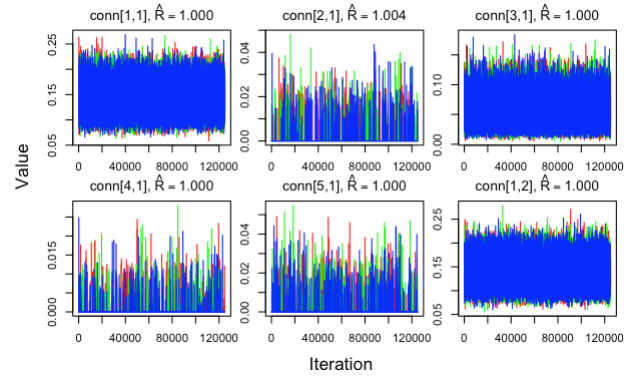
\includegraphics[width=8.81in]{./images/mcmc_chains1}

\textbf{Check goodness of fit}

In \emph{mignette}, we implement a posterior predictive check using the Freeman-Tukey discrepancy statistic to compare the fit of the observed data to simulated data from the model, following the guidelines of \href{https://doi.org/10.1002/ecm.1314}{Conn et al.~(2018)}. In the network model output, the posterior predictive check parameters are: 1) FT.obs = the Freeman-Tukey statistic for observed data, and 2) FT.rep = the Freeman-Tukey statistic for simulated data. The function \texttt{get\_FT\_fit()} produces a density plot of the Freeman-Tukey statistics for qualitatively comparing observed and simulated data, as well as outputting the Bayesian p-value of the goodness of fit based on these distributions. Very small (\textless0.05) or large (\textgreater0.95) Bayesian p-values suggest a lack of fit of the model. For a full discussion of checking Bayesian models, see Conn et al.~(2018).

We can then look at the posterior predictive check of the American Redstart mode using the code below, which shows largely overlapping distributions of the Freeman-Tukey discrepancy statistics for the observed and simulated data, with a corresponding Bayesian p-value of 0.58 - indicating sufficient goodness of fit.

\begin{Shaded}
\begin{Highlighting}[]
\FunctionTok{get\_FT\_fit}\NormalTok{(network\_model)}
\end{Highlighting}
\end{Shaded}

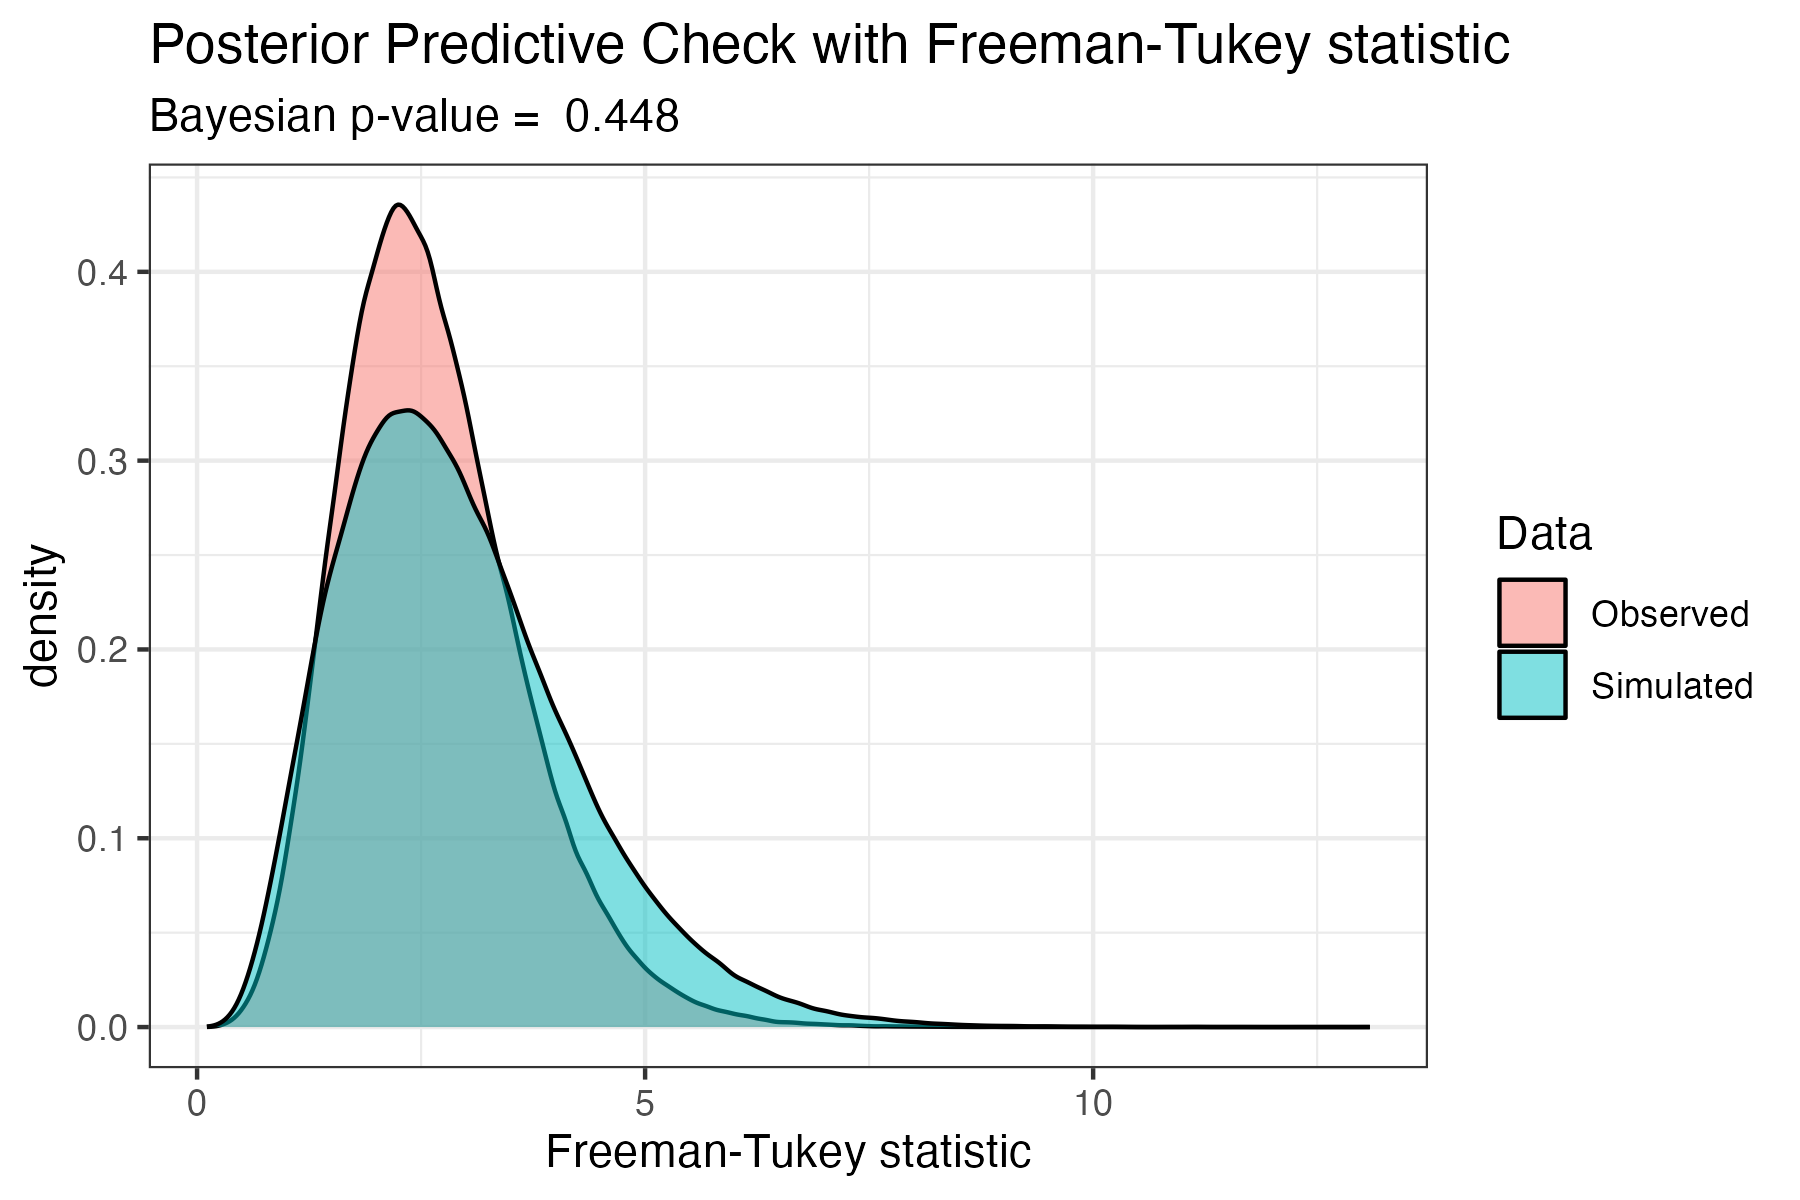
\includegraphics[width=25in]{./images/p.fit}

\textbf{Uncertainty in the connectivity estimates}

The network model output provides credible intervals in addition to the mean of the connectivity estimates. Uncertainty in the network connectivity estimates is characterized by the credible intervals provided in the network model output for the conn\_g parameter. The mignette function \texttt{plot\_network\_CI()} plots the mean and 95\% credible intervals for network connectivity which allows users to assess the uncertainty in the estimates.

\begin{verbatim}
plot_network_CI(network_model = network_model, stage = “Breeding”, 
stage_colors = brnode_colors, overlap = TRUE)
\end{verbatim}

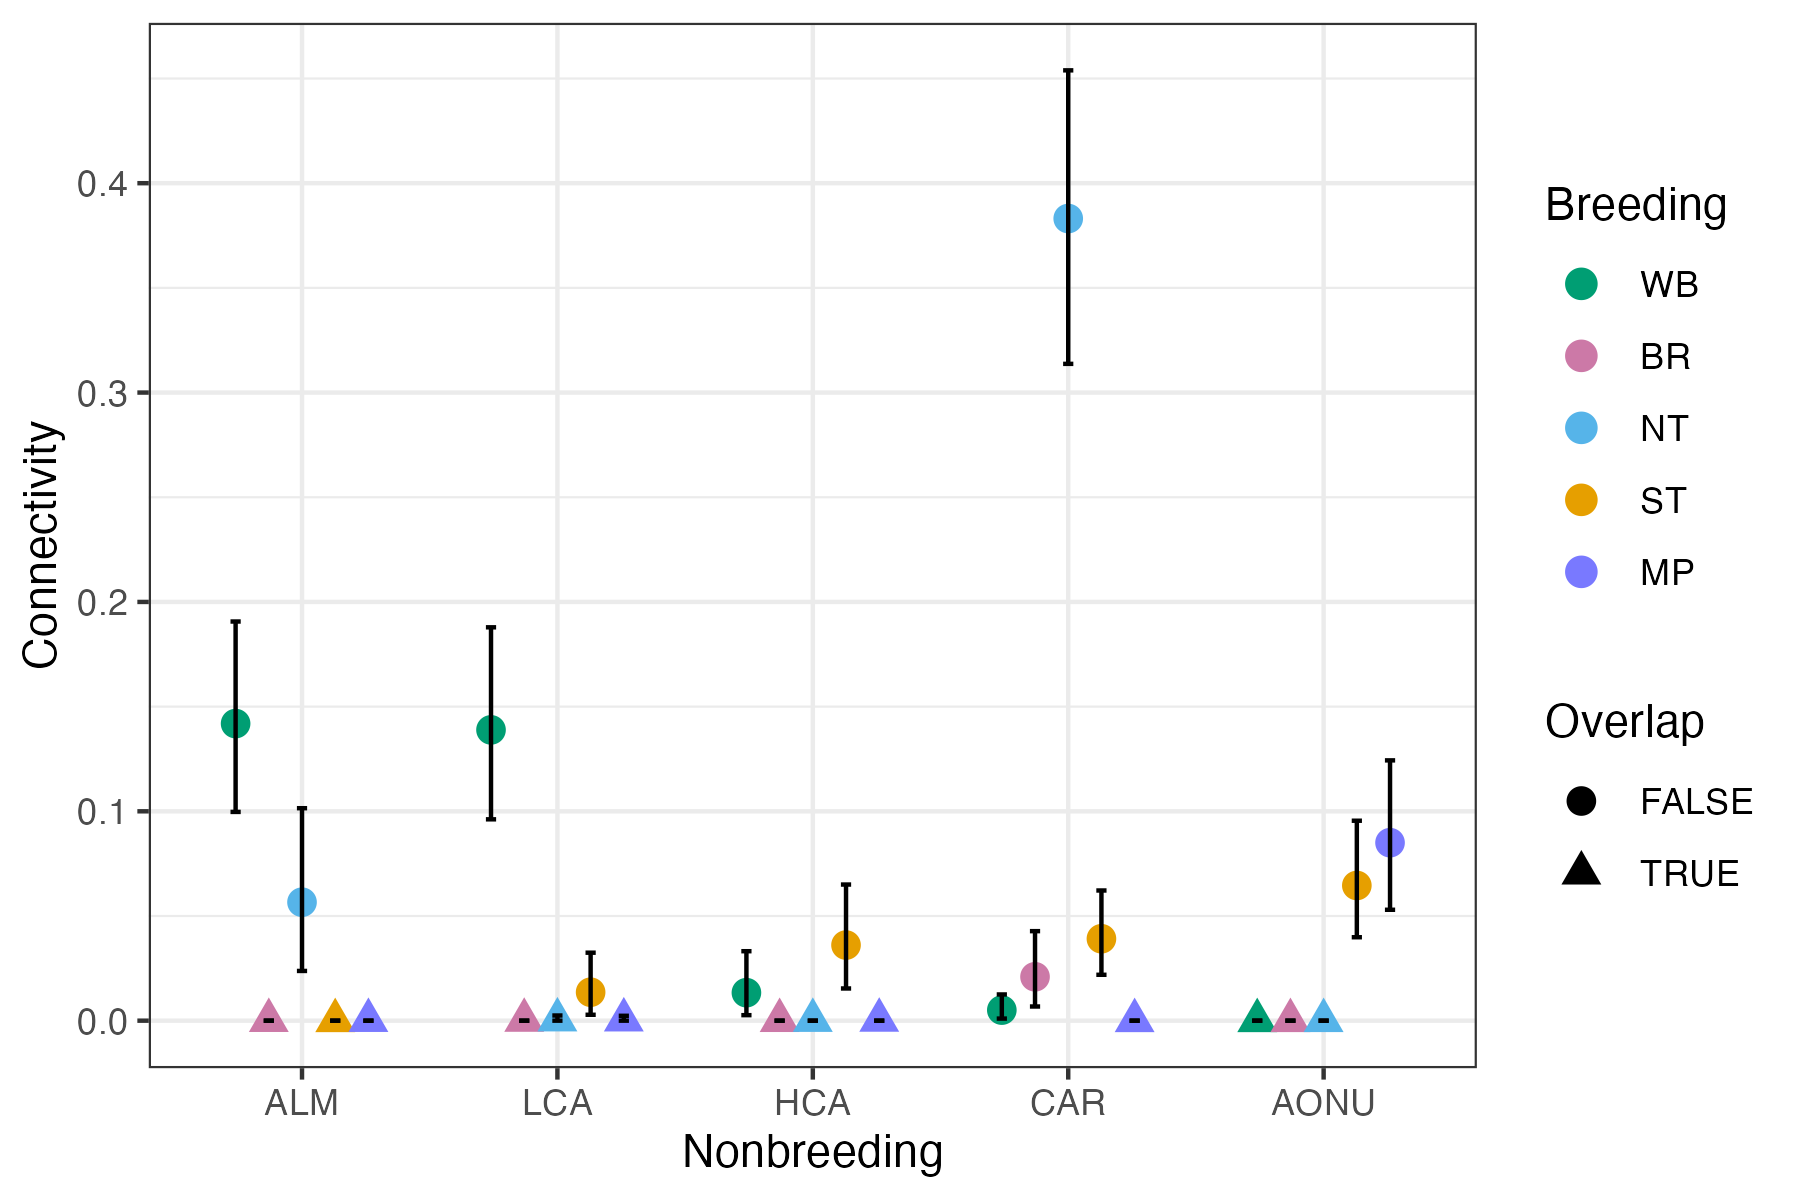
\includegraphics[width=25in]{./images/p.ci}

\textbf{Visualize network}

The raw connectivity matrix is used to plot the network. We plot the migratory network with the provided \texttt{mignette} functions \texttt{net\_create()} and \texttt{net\_draw()}. We set \texttt{connected\_tol\ =\ 0.01} which plots only the edges with connectivity values of greater than 0.01.

\begin{Shaded}
\begin{Highlighting}[]
\NormalTok{amre\_net }\OtherTok{\textless{}{-}} \FunctionTok{net\_create}\NormalTok{(}\AttributeTok{network\_model =}\NormalTok{ network\_model,}
                       \AttributeTok{margin =} \FloatTok{0.05}\NormalTok{)}
\CommentTok{\#set the display size range for nodes (min and max), default 1{-}10}
\NormalTok{amre\_net}\SpecialCharTok{$}\NormalTok{display\_par}\SpecialCharTok{$}\NormalTok{node\_size\_scale }\OtherTok{\textless{}{-}} \FunctionTok{c}\NormalTok{(}\DecValTok{8}\NormalTok{,}\DecValTok{25}\NormalTok{)}
\CommentTok{\#set the display size range for edges (min and max), default 1{-}10}
\NormalTok{amre\_net}\SpecialCharTok{$}\NormalTok{display\_par}\SpecialCharTok{$}\NormalTok{edge\_size\_scale }\OtherTok{\textless{}{-}} \FunctionTok{c}\NormalTok{(}\DecValTok{1}\NormalTok{,}\DecValTok{5}\NormalTok{)}
\CommentTok{\# change colors}
\NormalTok{amre\_net}\SpecialCharTok{$}\NormalTok{display\_par}\SpecialCharTok{$}\NormalTok{brnode\_colors }\OtherTok{\textless{}{-}} \FunctionTok{c}\NormalTok{(}\StringTok{"\#009e73"}\NormalTok{, }\StringTok{"\#cc79a7"}\NormalTok{, }\StringTok{"\#56b4e9"}\NormalTok{, }\StringTok{"\#e69f00"}\NormalTok{, }\StringTok{"\#7979ff"}\NormalTok{)}
\NormalTok{amre\_net}\SpecialCharTok{$}\NormalTok{display\_par}\SpecialCharTok{$}\NormalTok{nbnode\_colors }\OtherTok{\textless{}{-}} \StringTok{"grey80"}

\FunctionTok{net\_draw}\NormalTok{(amre\_net)}
\end{Highlighting}
\end{Shaded}

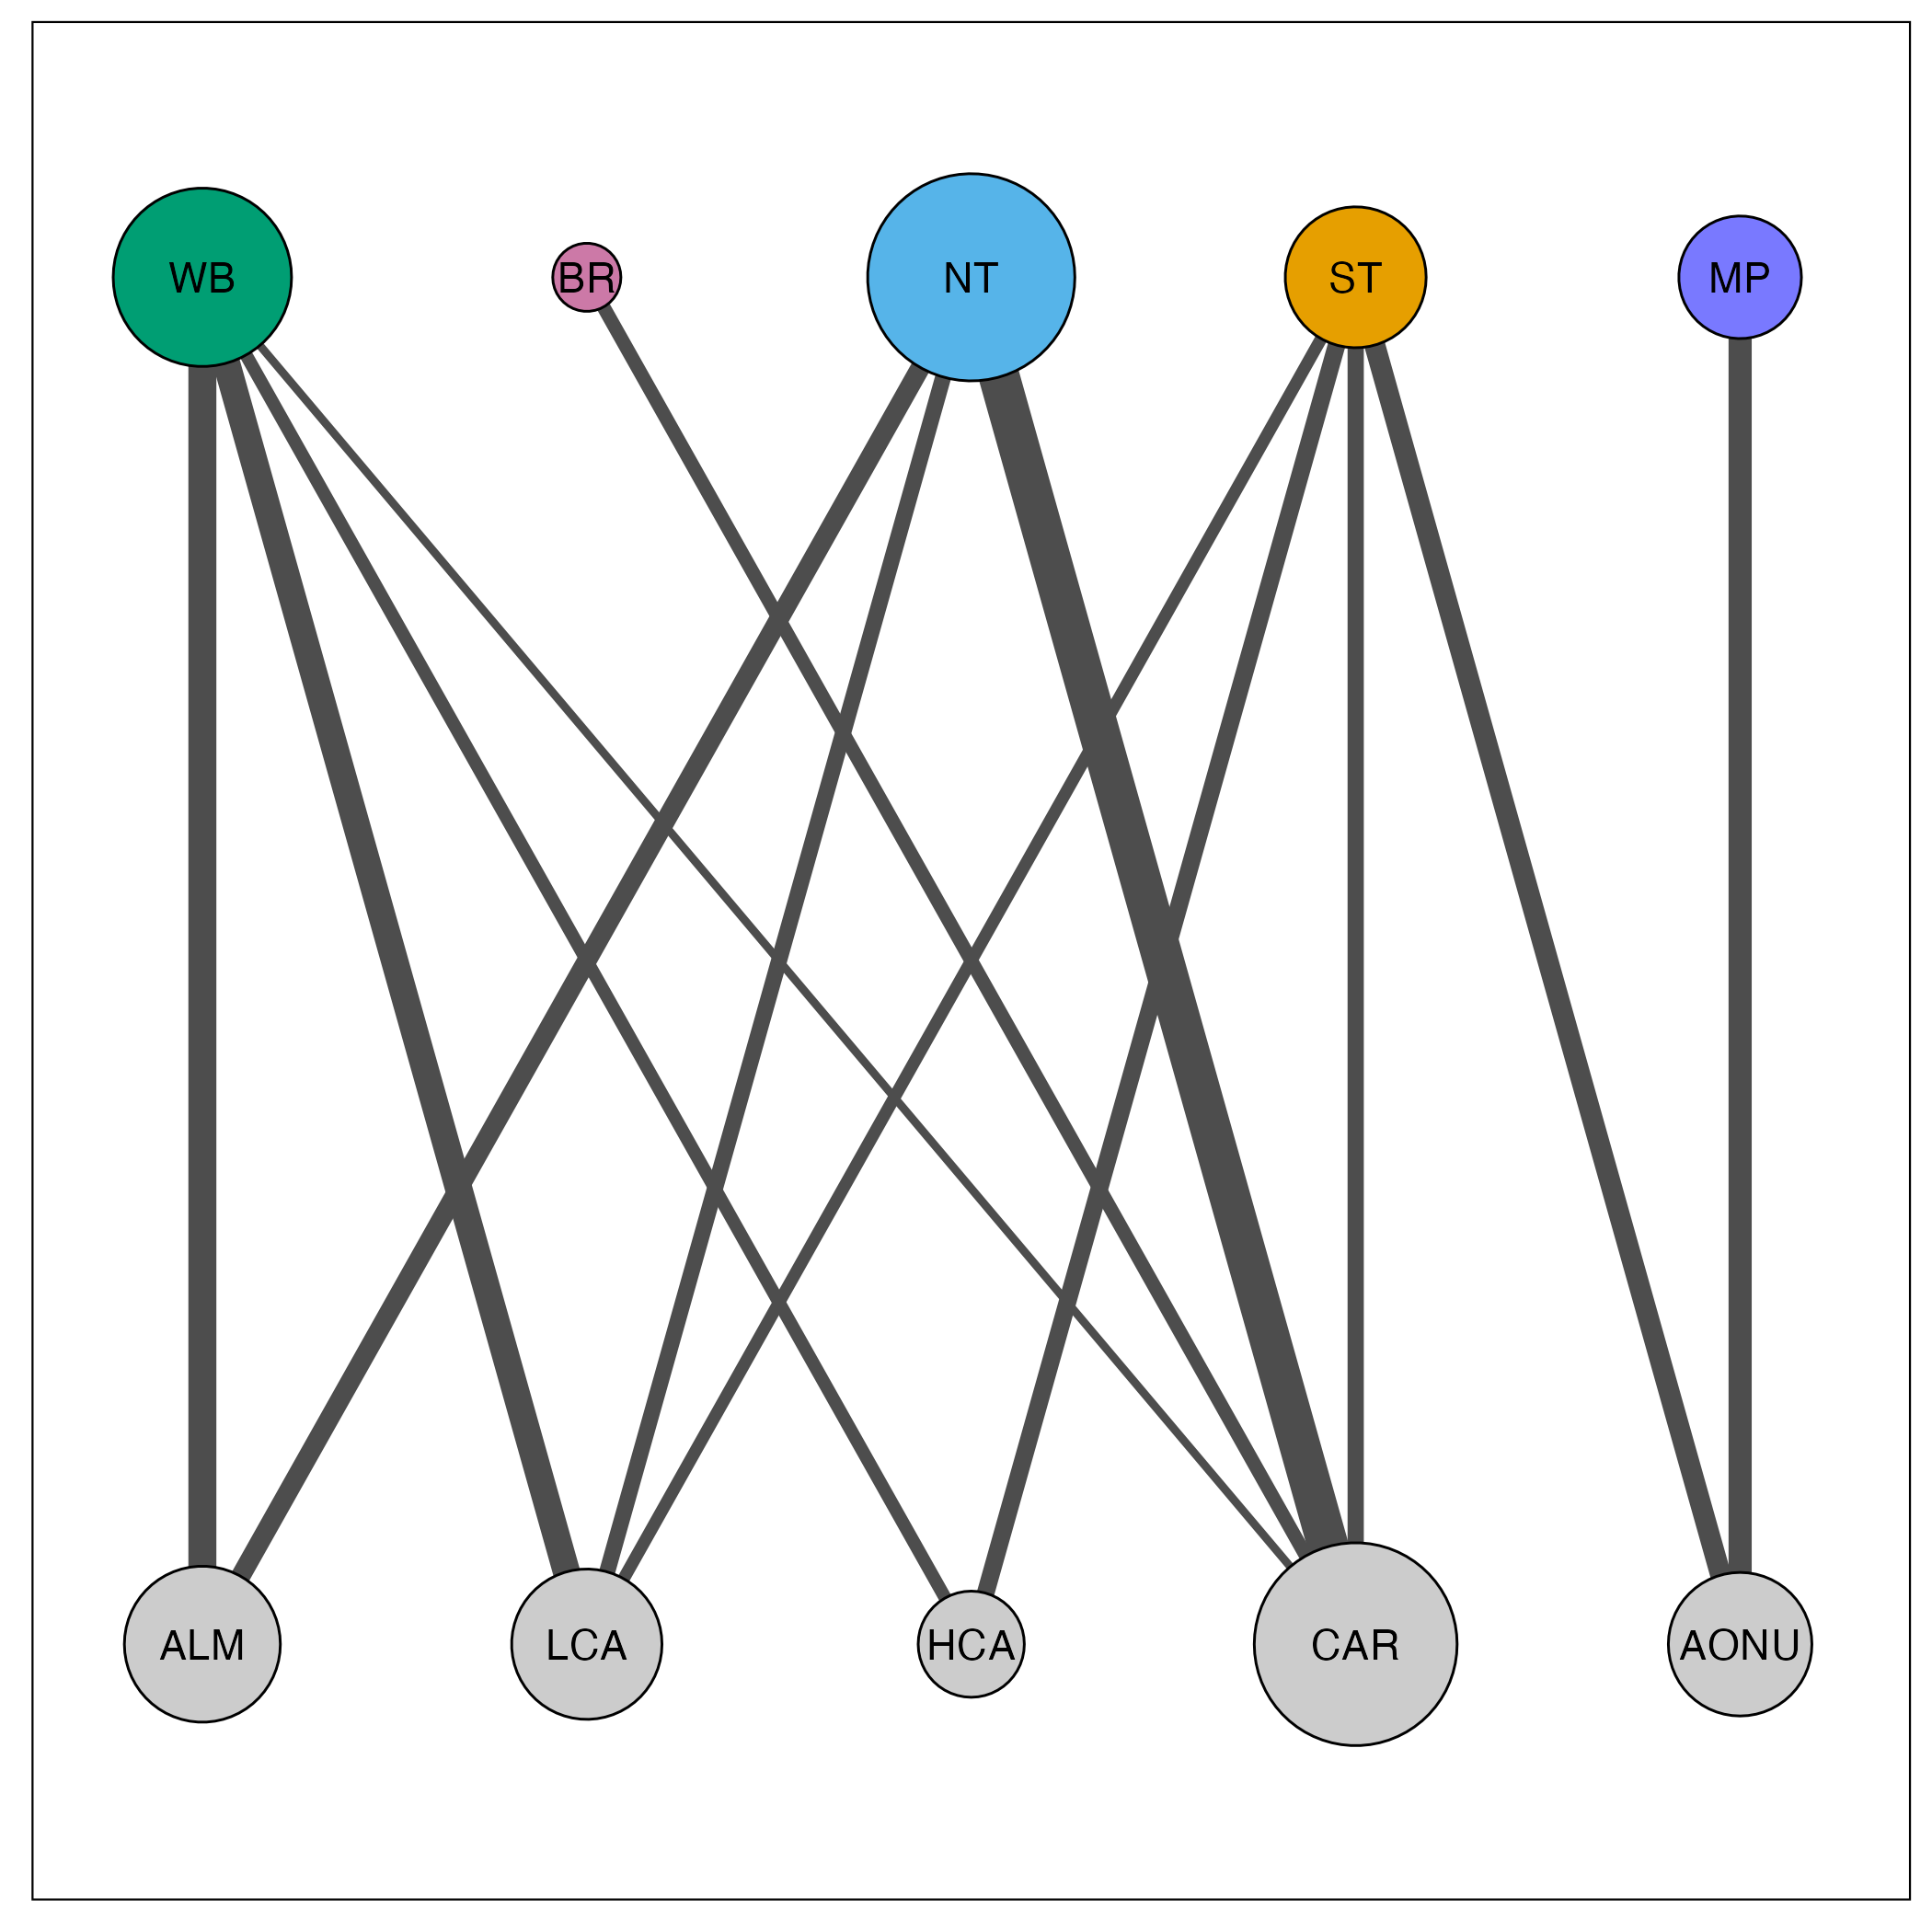
\includegraphics[width=29.17in]{./images/p.amre.net}

In this visualization, node size corresponds to the amount of connectivity with that population and edge size corresponds to the amount of connectivity between the populations. Breeding populations are in the top row, for which we provided custom colors, and nonbreeding populations are in the bottom row.

This sums up the basics of creating and visualizing a migratory network. We encourage users to explore and build upon the visualization tools we provide (e.g.~overlay the migratory networks on geographic ranges) - the options are endless, enjoy!

\hypertarget{nodes}{%
\chapter{Define breeding and nonbreeding nodes}\label{nodes}}

The first step of creating a migratory network is to spatially define the nodes (i.e.~populations) that make up the sampled portions of the breeding and nonbreeding range. This can either be done with \emph{vector} data for discrete spatial boundaries of nodes or \emph{raster} data for a continuous surface probabilistic membership of geographic cells to a node (e.g., population genetic structure of a genoscape \citep{ruegg2020genoscape}).

\begin{Shaded}
\begin{Highlighting}[]
\FunctionTok{library}\NormalTok{(mignette)}
\FunctionTok{library}\NormalTok{(tidyverse)}
\FunctionTok{library}\NormalTok{(terra)}
\end{Highlighting}
\end{Shaded}

\hypertarget{vector-data}{%
\section{Vector data}\label{vector-data}}

Vector data can define nodes by representing geographic boundaries such as political borders or biogeographic regions. In \texttt{mignette}, we provide data for \emph{conservation regions} of the Western Hemisphere that integrate geopolitical boundaries and ecoregions.

\begin{Shaded}
\begin{Highlighting}[]
\CommentTok{\# SpatVector from terra package}
\NormalTok{regions\_file }\OtherTok{\textless{}{-}} \FunctionTok{system.file}\NormalTok{(}\StringTok{"extdata"}\NormalTok{, }\StringTok{"conservation\_regions.Rds"}\NormalTok{, }\AttributeTok{package =} \StringTok{"mignette"}\NormalTok{)}
\CommentTok{\# read in file as SpatVector}
\NormalTok{conservation\_regions }\OtherTok{\textless{}{-}}\NormalTok{ terra}\SpecialCharTok{::}\FunctionTok{vect}\NormalTok{(regions\_file)}

\NormalTok{terra}\SpecialCharTok{::}\FunctionTok{plot}\NormalTok{(conservation\_regions, }\AttributeTok{col=}\FunctionTok{rainbow}\NormalTok{(}\DecValTok{10}\NormalTok{))}
\end{Highlighting}
\end{Shaded}

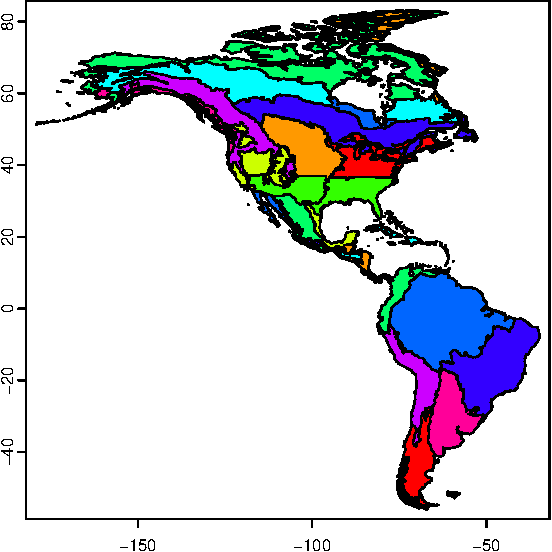
\includegraphics{Mignette_files/figure-latex/unnamed-chunk-11-1.pdf}

For defining a node, we are only interested in regions that we have data. It's straightforward with the spatial functions from \texttt{terra} to determine the sampled regions. Here, we find the conservation regions for which we have sampled American Redstart data from the nonbreeding range.

\begin{Shaded}
\begin{Highlighting}[]
\CommentTok{\# create SpatVector points object from Redstart lat/lon sampling data}
\NormalTok{nonbreeding\_coords }\OtherTok{\textless{}{-}}\NormalTok{ terra}\SpecialCharTok{::}\FunctionTok{vect}\NormalTok{(mignette}\SpecialCharTok{::}\NormalTok{amre\_nonbreeding\_data, }
                             \AttributeTok{geom=}\FunctionTok{c}\NormalTok{(}\StringTok{"Lon"}\NormalTok{, }\StringTok{"Lat"}\NormalTok{),}
                             \AttributeTok{crs =} \StringTok{"EPSG:4326"}\NormalTok{)}
\CommentTok{\# find spatial intersection of points with conservation regions}
\NormalTok{sampled\_conservation\_regions }\OtherTok{\textless{}{-}}\NormalTok{ terra}\SpecialCharTok{::}\FunctionTok{intersect}\NormalTok{(nonbreeding\_coords,}
\NormalTok{                                        conservation\_regions)}
\CommentTok{\# count the number of sampled individuals associated with each conservation region}
\NormalTok{sampled\_table }\OtherTok{\textless{}{-}} \FunctionTok{table}\NormalTok{(sampled\_conservation\_regions}\SpecialCharTok{$}\NormalTok{Region)}
\NormalTok{sampled\_table}
\end{Highlighting}
\end{Shaded}

\begin{verbatim}
## 
## Amazon/Orinoco-Northern Uplands         Atlantic Lowland Mexico 
##                              20                              16 
##                       Caribbean        Highland Central America 
##                              52                               5 
##         Lowland Central America 
##                              17
\end{verbatim}

Downstream in the workflow, we need sufficiently sampling of individuals in (or inference to) a node. So, we'll only retain the conservation regions with more than 3 samples\ldots here, that is all of them:

\begin{Shaded}
\begin{Highlighting}[]
\CommentTok{\# retain conservation region names with more than 3 samples}
\NormalTok{retained\_regions }\OtherTok{\textless{}{-}} \FunctionTok{names}\NormalTok{(sampled\_table[sampled\_table }\SpecialCharTok{\textgreater{}} \DecValTok{3}\NormalTok{])}
\NormalTok{retained\_regions}
\end{Highlighting}
\end{Shaded}

\begin{verbatim}
## [1] "Amazon/Orinoco-Northern Uplands" "Atlantic Lowland Mexico"        
## [3] "Caribbean"                       "Highland Central America"       
## [5] "Lowland Central America"
\end{verbatim}

Thus, we've identified the 5 nonbreeding nodes for the American Redstart data: Amazon/Orinoco-Northern Uplands (AONU), Atlantic Lowland Mexico (ALM), Caribbean (CAR), Highland Central America (HCA), and Lowland Central America (LCA). We can plot these conservation regions along with the corresponding sampling points.

\begin{Shaded}
\begin{Highlighting}[]
\CommentTok{\# subset conservation regions file by retained regions}
\NormalTok{conservation\_regions\_subset }\OtherTok{\textless{}{-}}\NormalTok{ terra}\SpecialCharTok{::}\FunctionTok{subset}\NormalTok{(conservation\_regions, }
\NormalTok{                                             conservation\_regions}\SpecialCharTok{$}\NormalTok{Region }\SpecialCharTok{\%in\%}\NormalTok{ retained\_regions)}

\CommentTok{\# plot}
\NormalTok{ggplot2}\SpecialCharTok{::}\FunctionTok{ggplot}\NormalTok{() }\SpecialCharTok{+}
\NormalTok{  tidyterra}\SpecialCharTok{::}\FunctionTok{geom\_spatvector}\NormalTok{(}\AttributeTok{data =}\NormalTok{ conservation\_regions\_subset, ggplot2}\SpecialCharTok{::}\FunctionTok{aes}\NormalTok{(}\AttributeTok{fill =}\NormalTok{ Region)) }\SpecialCharTok{+}
\NormalTok{  tidyterra}\SpecialCharTok{::}\FunctionTok{geom\_spatvector}\NormalTok{(}\AttributeTok{data =}\NormalTok{ nonbreeding\_coords) }\SpecialCharTok{+}
\NormalTok{  ggplot2}\SpecialCharTok{::}\FunctionTok{theme\_bw}\NormalTok{()}
\end{Highlighting}
\end{Shaded}

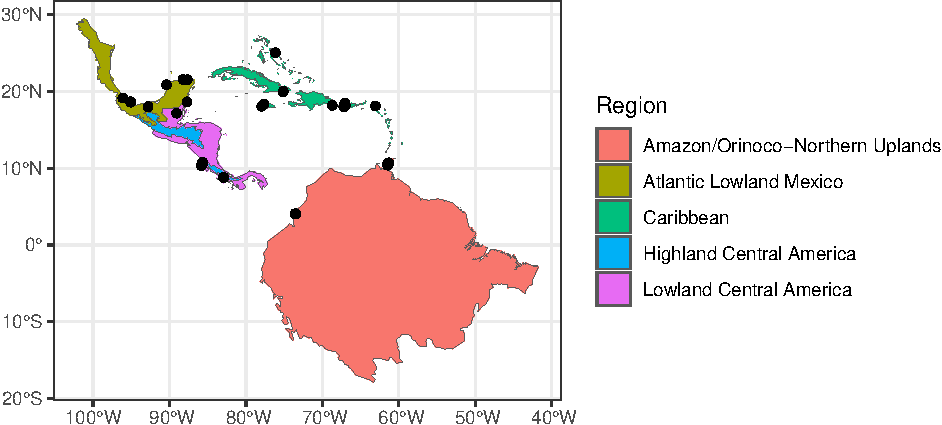
\includegraphics{Mignette_files/figure-latex/unnamed-chunk-14-1.pdf}

\hypertarget{raster-data}{%
\section{Raster data}\label{raster-data}}

Raster data is used when populations are defined by a continuous surface of probabilities of membership to a population. In the example here, we have population genetic data from the American Redstart that define breeding populations (i.e., American Redstart genoscape, \citep{desaix2023low}). We have defined these nodes as Western Boreal (WB), Basin Rockies (BR), Northern Temperate (NT), Southern Temperate (ST) and Maritime Provinces (MP). Raster data for nodes are used in \texttt{mignette} to get node abundance that is scaled by the raster probabilities of population membership, as shown in the next section.

\begin{Shaded}
\begin{Highlighting}[]
\NormalTok{amre\_genoscape\_file }\OtherTok{\textless{}{-}} \FunctionTok{system.file}\NormalTok{(}\StringTok{"extdata"}\NormalTok{, }\StringTok{"amre\_genoscape.Rds"}\NormalTok{, }\AttributeTok{package =} \StringTok{"mignette"}\NormalTok{)}
\NormalTok{amre\_genoscape }\OtherTok{\textless{}{-}}\NormalTok{ terra}\SpecialCharTok{::}\FunctionTok{rast}\NormalTok{(amre\_genoscape\_file)}
\NormalTok{terra}\SpecialCharTok{::}\FunctionTok{plot}\NormalTok{(amre\_genoscape)}
\end{Highlighting}
\end{Shaded}

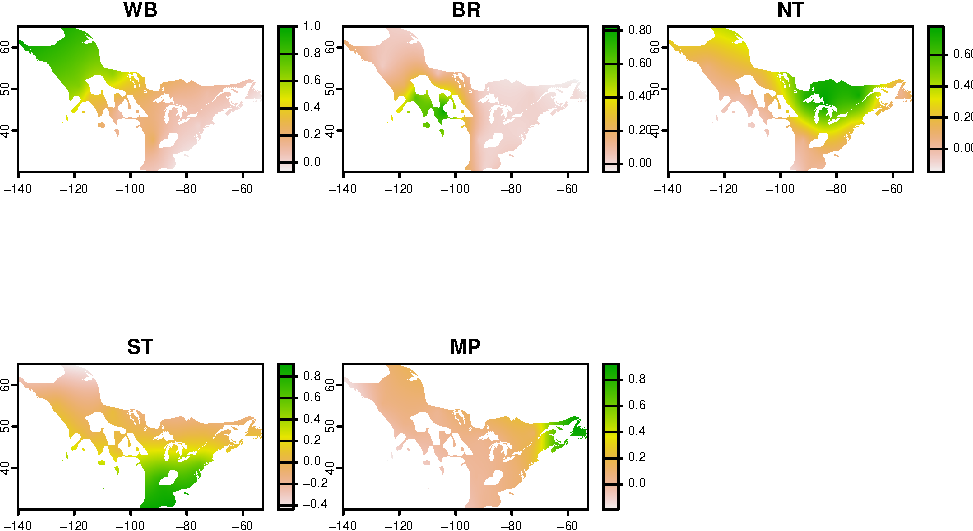
\includegraphics{Mignette_files/figure-latex/unnamed-chunk-15-1.pdf}

While it is outside the scope of \texttt{mignette} to perform the requisite population genetics analyses for producing these rasters, users with genetic data and expertise with genetic clustering analyses may be interested in the \protect\hyperlink{supplemental}{Supplementary information} that provide additional information and code.

Now on to \protect\hyperlink{data}{Step 2) Abundance and migratory connectivity data}

\hypertarget{data}{%
\chapter{Assemble abundance and migratory connectivity data}\label{data}}

The two main data inputs into the migratory network model are \emph{abundance data} and \emph{migratory connectivity data} for the nodes.

\hypertarget{abundance-data}{%
\section{Abundance data}\label{abundance-data}}

Once users have defined breeding and nonbreeding nodes for their sampled data, the species' abundance for each node is needed. In some cases, users may be using node definitions for which abundance estimates have already been calculated. Regardless of however \texttt{mignette} users obtain abundance data for the breeding and nonbreeding nodes, it needs to be formatted in the following manner for using with \texttt{mignette} as shown with the example American Redstart data:

\begin{Shaded}
\begin{Highlighting}[]
\NormalTok{mignette}\SpecialCharTok{::}\NormalTok{amre\_abundance}
\end{Highlighting}
\end{Shaded}

\begin{tabular}{l|r}
\hline
Population & Relative\_abundance\\
\hline
BR & 2403\\
\hline
ST & 9419\\
\hline
MP & 19011\\
\hline
NT & 72147\\
\hline
WB & 26080\\
\hline
HCA & 326\\
\hline
AONU & 1139\\
\hline
LCA & 2802\\
\hline
ALM & 3169\\
\hline
CAR & 7987\\
\hline
\end{tabular}

where the first column of the data frame is the node (i.e., population) and the second column is the abundance. All sampled nodes from the breeding and nonbreeding range need to be present in this file.

One common form of abundance data is as a raster where each cell specifies abundance (for example \href{https://science.ebird.org/en/status-and-trends}{eBird Status and Trends data} available from the \href{https://cornelllabofornithology.github.io/ebirdst/}{ebirdst R package}). If you are working with raster abundance data and need to summarize it at the node level, there are two functions in \texttt{mignette} to facilitate that process.

\begin{enumerate}
\def\labelenumi{\arabic{enumi}.}
\item
  \texttt{get\_vector\_abunds(populations,\ abunds)} - sums the abundance data for a SpatRaster object of abundance (specified by the \texttt{abunds} parameter) by the vector node delineation (specified by the \texttt{populations} parameter).
\item
  \texttt{get\_raster\_abunds(populations,\ abunds)} - sums the abundance data for a SpatRaster object of abundance by \emph{weighting} values based on the raster node delineation.
\end{enumerate}

\hypertarget{migratory-connectivity-data}{%
\section{Migratory connectivity data}\label{migratory-connectivity-data}}

In addition to having node abundance data, \texttt{mignette} users need to have migratory connectivity data detailing the number of individuals connecting the nodes between the two stages. Migratory connectivity data has a directionality to it - i.e., there is an ``encounter'' season and a ``recovery'' season - and we use this corresponding terminology from \citep{prochazka2017delineating}. In \texttt{mignette} different types of migratory connectivity data use different models based on whether the breeding or nonbreeding seasons are the ``encounter'' or ``recovery'' seasons. To account for users providing different types of connectivity data, we provide three different models in mignette: 1 = the nonbreeding season is ``encounter'' and the breeding season is ``recovery''; 2 = the breeding season is ``encounter'' and the nonbreeding season is ``recovery''; and 3 = connectivity data are from both model types 1 and 2. For cross-season mark-recapture data (i.e.~from banding or geolocators), the encounter season is where the individual is captured and the recovery season is where they are re-captured or re-sighted or, in the case of geolocator data, inferred to have originated. For genetic data, the encounter season is nonbreeding and the recovery season is breeding (i.e., ``inferred'').

The American Redstart assignment is all from genetic data \citep{desaix2023low}:

\begin{Shaded}
\begin{Highlighting}[]
\NormalTok{mignette}\SpecialCharTok{::}\NormalTok{amre\_assign}
\end{Highlighting}
\end{Shaded}

\begin{tabular}{l|r|r|r|r|r}
\hline
Breeding & CAR & AONU & ALM & LCA & HCA\\
\hline
BR & 1 & 0 & 0 & 0 & 0\\
\hline
MP & 0 & 9 & 0 & 0 & 0\\
\hline
NT & 58 & 0 & 3 & 1 & 0\\
\hline
ST & 9 & 12 & 0 & 1 & 4\\
\hline
WB & 1 & 0 & 20 & 15 & 1\\
\hline
\end{tabular}

For the \texttt{mignette} migratory network, the migratory connectivity data needs to be formatted as above: where the first column provides the node names from the ``recovery'' season in the rows and the remaining columns are the ``encounter'' season node names. The values in the data frame all the numbers of individuals assigned from the ``encounter'' season to the ``recovery'' season (in this case, American Redstarts assigned from the nonbreeding sampling location to the breeding population).

Thus, when \texttt{mignette} users have migratory connectivity data types that include assignment in both directions, they will need to create two separate data frames for those data.

Now on to \protect\hyperlink{model}{Step 3) Modeling the migratory network}

\hypertarget{model}{%
\chapter{Modeling the migratory network}\label{model}}

\hypertarget{input-data}{%
\section{Input data}\label{input-data}}

As described in the previous section the data required are:

\begin{itemize}
\tightlist
\item
  Abundance
\item
  Migratory connectivity
\end{itemize}

The abundance data need to be in the following format, with node IDs (same names as in the \emph{assignment} file) in the first column and abundance values in the second column.

\begin{tabular}{l|r}
\hline
Population & Relative\_abundance\\
\hline
BR & 2403\\
\hline
ST & 9419\\
\hline
MP & 19011\\
\hline
NT & 72147\\
\hline
WB & 26080\\
\hline
HCA & 326\\
\hline
AONU & 1139\\
\hline
LCA & 2802\\
\hline
ALM & 3169\\
\hline
CAR & 7987\\
\hline
\end{tabular}

For the migratory connectivity data, the input data needs to correspond to the following format:

\begin{tabular}{l|r|r|r|r|r}
\hline
Breeding & CAR & AONU & ALM & LCA & HCA\\
\hline
BR & 1 & 0 & 0 & 0 & 0\\
\hline
MP & 0 & 9 & 0 & 0 & 0\\
\hline
NT & 58 & 0 & 3 & 1 & 0\\
\hline
ST & 9 & 12 & 0 & 1 & 4\\
\hline
WB & 1 & 0 & 20 & 15 & 1\\
\hline
\end{tabular}

If you skipped it, see the previous \protect\hyperlink{data}{Step 2) Abundance and migratory connectivity data} section for specific details on the input data formatting!

For the following functions, we specify the order of the nodes we are using for the model. Here, we are just ordering nodes geographically by longitude to facilitate straightforward interpretation of the output.

\begin{Shaded}
\begin{Highlighting}[]
\NormalTok{brnode\_names }\OtherTok{\textless{}{-}} \FunctionTok{c}\NormalTok{(}\StringTok{"WB"}\NormalTok{, }\StringTok{"BR"}\NormalTok{, }\StringTok{"NT"}\NormalTok{, }\StringTok{"ST"}\NormalTok{, }\StringTok{"MP"}\NormalTok{)}
\NormalTok{nbnode\_names }\OtherTok{\textless{}{-}} \FunctionTok{c}\NormalTok{(}\StringTok{"ALM"}\NormalTok{, }\StringTok{"LCA"}\NormalTok{, }\StringTok{"HCA"}\NormalTok{, }\StringTok{"CAR"}\NormalTok{, }\StringTok{"AONU"}\NormalTok{)}
\end{Highlighting}
\end{Shaded}

For the American Redstart migratory network, we use \texttt{model\ =\ 1} from \texttt{mignette} which specifies that nonbreeding nodes are ``encountered'' and breeding nodes are ``recovered'' (i.e., inferred). This output saves the model as \texttt{amre.genetic.model\_1.txt}. Below we specify \texttt{parallel\ =\ TRUE} to run MCMC on multiple cores and use the remaining defaults described previously CHANGE LINK. This step is computationally intensive and takes \textasciitilde2 minutes to run on a 2023 MacBook Pro with an Apple M2 Pro chip.

\begin{Shaded}
\begin{Highlighting}[]
\NormalTok{network\_model }\OtherTok{\textless{}{-}} \FunctionTok{run\_network\_model}\NormalTok{(}\AttributeTok{abundance =}\NormalTok{ amre\_abundance, }
                           \AttributeTok{nb2br\_assign =}\NormalTok{ amre\_assign,}
                           \AttributeTok{brnode\_names =}\NormalTok{ brnode\_names, }
                           \AttributeTok{nbnode\_names =}\NormalTok{ nbnode\_names,}
                           \AttributeTok{model =} \StringTok{"BR"}\NormalTok{, }\AttributeTok{base\_filename =} \StringTok{"amre.genetic"}\NormalTok{,}
                           \AttributeTok{parallel =} \ConstantTok{TRUE}\NormalTok{)}
\end{Highlighting}
\end{Shaded}

The \texttt{run\_network\_model()} function outputs a list object with four components. The first component of the output, \texttt{{[}{[}“conn”{]}{]}}, is an R tibble object of the mean connectivity estimated between nodes (Table 1). These values are interpreted as the proportion of individuals the global population that migrate between the corresponding populations, as such all of the values in the network matrix sum to one. The second component, \texttt{{[}{[}“jags\_out”{]}{]}}, is the full output from \texttt{jagsUI::autojags()} provided as a list object, which contains important model information such as parameter estimates and credible intervals, model specifications, and goodness of fit. The final two components, \texttt{{[}{[}“brnode\_names”{]}{]}} and \texttt{{[}{[}“nbnode\_names”{]}{]}}, store the node names corresponding to the rows and columns, respectively, of the connectivity matrix.

\begin{Shaded}
\begin{Highlighting}[]
\NormalTok{network\_model}\SpecialCharTok{$}\NormalTok{conn}
\end{Highlighting}
\end{Shaded}

\begin{tabular}{l|r|r|r|r|r}
\hline
Breeding & ALM & LCA & HCA & CAR & AONU\\
\hline
WB & 0.14422 & 0.13388 & 0.01340 & 0.00508 & 0.00002\\
\hline
BR & 0.00014 & 0.00019 & 0.00009 & 0.01655 & 0.00006\\
\hline
NT & 0.05010 & 0.02698 & 0.00011 & 0.38497 & 0.00005\\
\hline
ST & 0.00002 & 0.01126 & 0.03642 & 0.02810 & 0.06308\\
\hline
MP & 0.00011 & 0.00020 & 0.00023 & 0.00002 & 0.08470\\
\hline
\end{tabular}

The second component is the full output from \href{https://rdrr.io/cran/jagsUI/man/autojags.html}{\texttt{*jagsUI*\ autojags()}} and is accessed by \texttt{network\_model\$jags\_out}.

We plot the migratory network with the provided \texttt{mignette} functions \texttt{net\_create()} and \texttt{net\_draw()}. We set \texttt{connected\_tol\ =\ 0.01} which plots only the edges with connectivity values of greater than 0.01. We also demonstrate below how to change parameters such as the colors and the node and edge scale size.

\begin{Shaded}
\begin{Highlighting}[]
\NormalTok{amre\_net }\OtherTok{\textless{}{-}} \FunctionTok{net\_create}\NormalTok{(}\AttributeTok{network\_model =}\NormalTok{ network\_model,}
                       \AttributeTok{margin =} \FloatTok{0.05}\NormalTok{)}
\CommentTok{\#set the display size range for nodes (min and max), default 1{-}10}
\NormalTok{amre\_net}\SpecialCharTok{$}\NormalTok{display\_par}\SpecialCharTok{$}\NormalTok{node\_size\_scale }\OtherTok{\textless{}{-}} \FunctionTok{c}\NormalTok{(}\DecValTok{8}\NormalTok{,}\DecValTok{25}\NormalTok{)}
\CommentTok{\#set the display size range for edges (min and max), default 1{-}10}
\NormalTok{amre\_net}\SpecialCharTok{$}\NormalTok{display\_par}\SpecialCharTok{$}\NormalTok{edge\_size\_scale }\OtherTok{\textless{}{-}} \FunctionTok{c}\NormalTok{(}\DecValTok{1}\NormalTok{,}\DecValTok{5}\NormalTok{)}
\CommentTok{\# change colors}
\NormalTok{amre\_net}\SpecialCharTok{$}\NormalTok{display\_par}\SpecialCharTok{$}\NormalTok{brnode\_colors }\OtherTok{\textless{}{-}} \FunctionTok{c}\NormalTok{(}\StringTok{"\#009e73"}\NormalTok{, }\StringTok{"\#cc79a7"}\NormalTok{, }\StringTok{"\#56b4e9"}\NormalTok{, }\StringTok{"\#e69f00"}\NormalTok{, }\StringTok{"\#7979ff"}\NormalTok{)}
\NormalTok{amre\_net}\SpecialCharTok{$}\NormalTok{display\_par}\SpecialCharTok{$}\NormalTok{nbnode\_colors }\OtherTok{\textless{}{-}} \StringTok{"grey80"}

\FunctionTok{net\_draw}\NormalTok{(amre\_net)}
\end{Highlighting}
\end{Shaded}

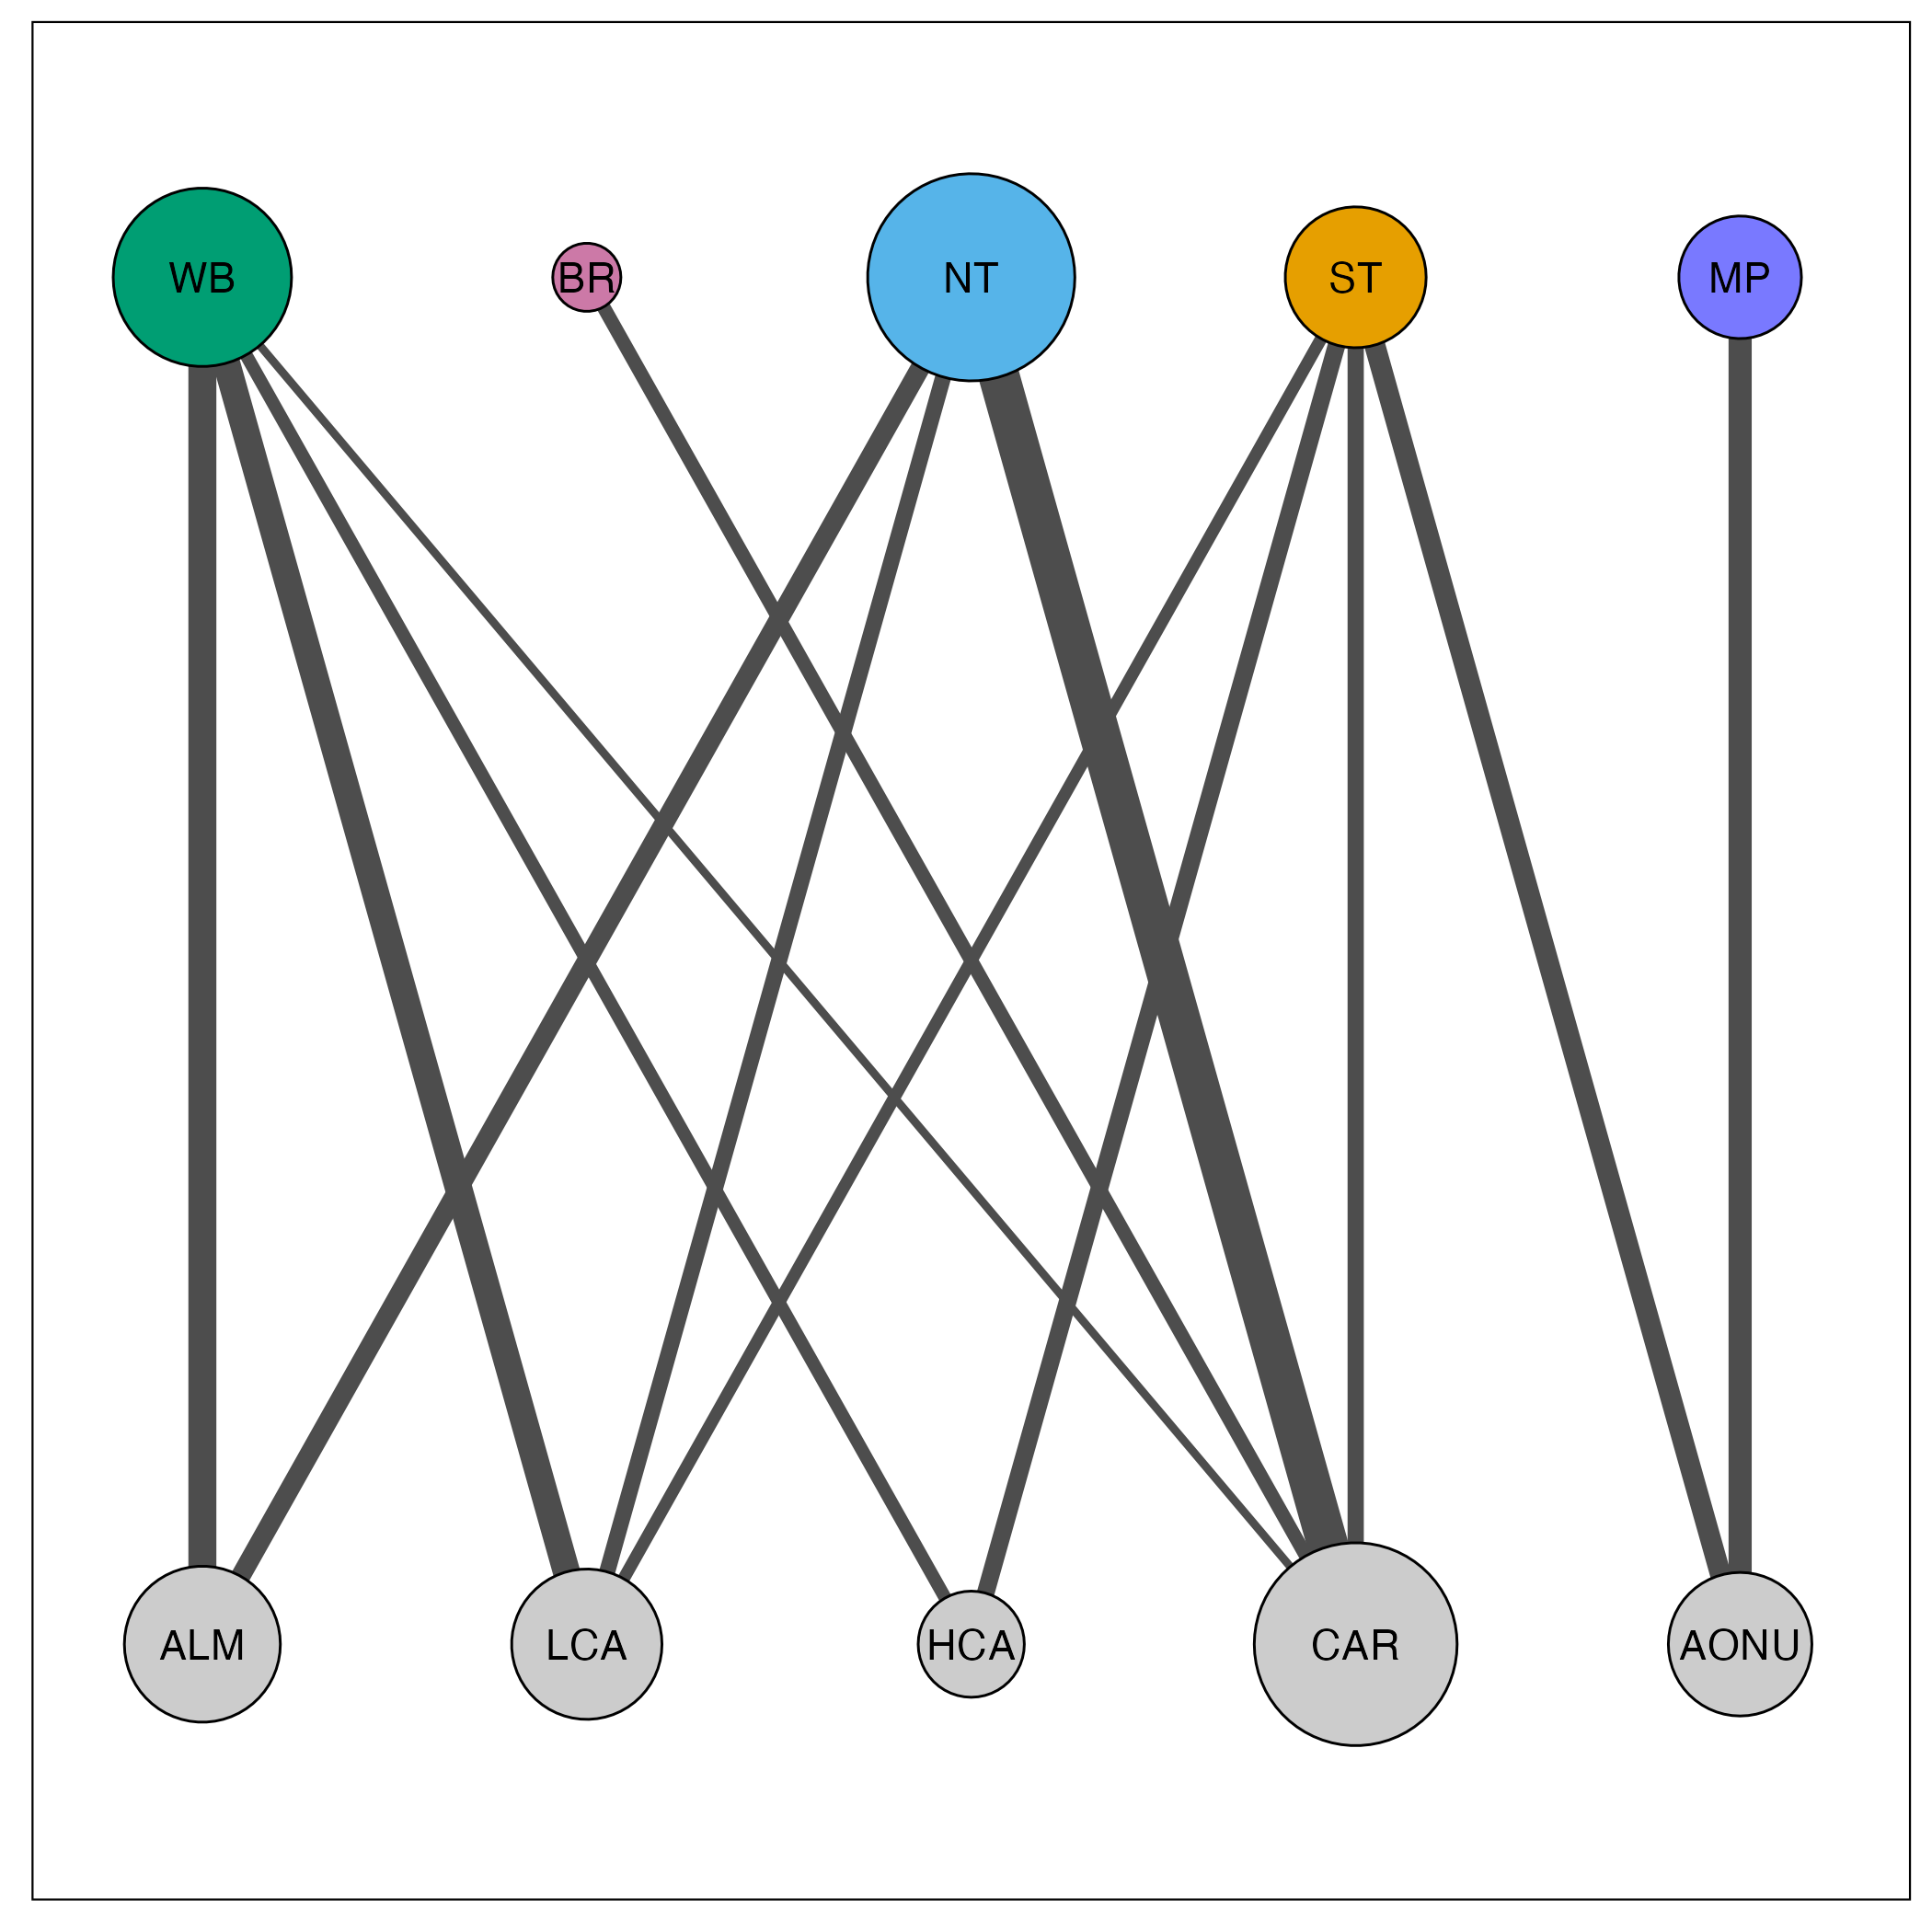
\includegraphics[width=29.17in]{./images/p.amre.net}

In this visualization, node size corresponds to the amount of connectivity with that population and edge size corresponds to the amount of connectivity between the populations. Breeding populations are in the top row, for which we provided custom colors, and nonbreeding populations are in the bottom row.

Now you have a migratory network! Check out the \protect\hyperlink{visualization}{visualization supplement} for additional ideas on plotting the network.

\hypertarget{visualization}{%
\chapter{Supplement: Visualizations}\label{visualization}}

\hypertarget{alluvial-plot}{%
\section{Alluvial plot}\label{alluvial-plot}}

Ok, we'll toss out another way to visualize these networks using the \href{https://cran.r-project.org/web/packages/ggalluvial/vignettes/ggalluvial.htm}{\texttt{ggalluvial} package} because it's really fun. In this alluvial plot, the width of the connections correspond to the network model connectivity output, thus correspond to the proportion of the global species abundance that use that migratory network. The bars on the top row are the breeding nodes scaled by abundance and the bottom row are the nonbreeding nodes scaled by abundance.

\begin{Shaded}
\begin{Highlighting}[]
\FunctionTok{library}\NormalTok{(tidyverse)}
\FunctionTok{library}\NormalTok{(mignette)}
\FunctionTok{library}\NormalTok{(ggalluvial)}

\NormalTok{brnode\_names }\OtherTok{\textless{}{-}} \FunctionTok{c}\NormalTok{(}\StringTok{"WB"}\NormalTok{, }\StringTok{"BR"}\NormalTok{, }\StringTok{"NT"}\NormalTok{, }\StringTok{"ST"}\NormalTok{, }\StringTok{"MP"}\NormalTok{)}
\NormalTok{nbnode\_names }\OtherTok{\textless{}{-}} \FunctionTok{c}\NormalTok{(}\StringTok{"ALM"}\NormalTok{, }\StringTok{"LCA"}\NormalTok{, }\StringTok{"HCA"}\NormalTok{, }\StringTok{"CAR"}\NormalTok{, }\StringTok{"AONU"}\NormalTok{)}

\NormalTok{cluster\_colors }\OtherTok{\textless{}{-}}  \FunctionTok{c}\NormalTok{(}
  \StringTok{\textasciigrave{}}\AttributeTok{ST}\StringTok{\textasciigrave{}} \OtherTok{=} \StringTok{"\#e69f00"}\NormalTok{, }\CommentTok{\# orange/Southern Temperate}
  \StringTok{\textasciigrave{}}\AttributeTok{BR}\StringTok{\textasciigrave{}} \OtherTok{=} \StringTok{"\#cc79a7"}\NormalTok{, }\CommentTok{\# pink/Basin Rockies (BR)}
  \StringTok{\textasciigrave{}}\AttributeTok{NT}\StringTok{\textasciigrave{}} \OtherTok{=} \StringTok{"\#56b4e9"}\NormalTok{, }\CommentTok{\# light blue/Northern Temperate (NT)}
  \StringTok{\textasciigrave{}}\AttributeTok{WB}\StringTok{\textasciigrave{}} \OtherTok{=} \StringTok{"\#009e73"}\NormalTok{, }\CommentTok{\# green/Western Boreal (WB)}
  \StringTok{\textasciigrave{}}\AttributeTok{MP}\StringTok{\textasciigrave{}} \OtherTok{=} \StringTok{"\#7979ff"} \CommentTok{\# dark blue/Maritime Provinces (MP)}
\NormalTok{) }

\NormalTok{amre\_conn\_df }\OtherTok{\textless{}{-}}\NormalTok{ mignette}\SpecialCharTok{::}\NormalTok{amre\_conn }\SpecialCharTok{\%\textgreater{}\%}
  \FunctionTok{as\_tibble}\NormalTok{(}\AttributeTok{rownames =} \StringTok{"Breeding"}\NormalTok{) }\SpecialCharTok{\%\textgreater{}\%}
  \FunctionTok{pivot\_longer}\NormalTok{(}\AttributeTok{cols =}\NormalTok{ ALM}\SpecialCharTok{:}\NormalTok{AONU, }\AttributeTok{names\_to =} \StringTok{"Nonbreeding"}\NormalTok{, }\AttributeTok{values\_to =} \StringTok{"Connectivity"}\NormalTok{) }\SpecialCharTok{\%\textgreater{}\%}
  \FunctionTok{mutate}\NormalTok{(}\AttributeTok{Connectivity =} \FunctionTok{ifelse}\NormalTok{(Connectivity }\SpecialCharTok{\textless{}} \FloatTok{0.01}\NormalTok{, }\DecValTok{0}\NormalTok{, Connectivity)) }\SpecialCharTok{\%\textgreater{}\%}
  \FunctionTok{mutate}\NormalTok{(}\AttributeTok{Breeding =} \FunctionTok{factor}\NormalTok{(Breeding, }\AttributeTok{levels =} \FunctionTok{rev}\NormalTok{(brnode\_names)),}
         \AttributeTok{Nonbreeding =} \FunctionTok{factor}\NormalTok{(Nonbreeding, }\AttributeTok{levels =} \FunctionTok{rev}\NormalTok{(nbnode\_names)))}

\NormalTok{p.alluvial }\OtherTok{\textless{}{-}} \FunctionTok{ggplot}\NormalTok{(amre\_conn\_df,}
       \FunctionTok{aes}\NormalTok{(}\AttributeTok{y =}\NormalTok{ Connectivity, }\AttributeTok{axis1 =}\NormalTok{ Nonbreeding, }\AttributeTok{axis2 =}\NormalTok{ Breeding)) }\SpecialCharTok{+}
  \FunctionTok{geom\_alluvium}\NormalTok{(}\FunctionTok{aes}\NormalTok{(}\AttributeTok{fill =}\NormalTok{ Breeding), }\AttributeTok{width =} \DecValTok{1}\SpecialCharTok{/}\DecValTok{12}\NormalTok{) }\SpecialCharTok{+}
  \FunctionTok{scale\_fill\_manual}\NormalTok{(}\AttributeTok{values =}\NormalTok{ cluster\_colors) }\SpecialCharTok{+}
  \FunctionTok{geom\_stratum}\NormalTok{(}\AttributeTok{alpha =} \FloatTok{0.25}\NormalTok{, }\AttributeTok{width =} \DecValTok{1}\SpecialCharTok{/}\DecValTok{12}\NormalTok{) }\SpecialCharTok{+}
  \FunctionTok{geom\_text}\NormalTok{(}\AttributeTok{stat =} \StringTok{"stratum"}\NormalTok{, }\FunctionTok{aes}\NormalTok{(}\AttributeTok{label =} \FunctionTok{after\_stat}\NormalTok{(stratum))) }\SpecialCharTok{+}
  \FunctionTok{scale\_x\_discrete}\NormalTok{(}\AttributeTok{limits =} \FunctionTok{c}\NormalTok{(}\StringTok{"Nonbreeding"}\NormalTok{, }\StringTok{"Breeding"}\NormalTok{),}
                   \AttributeTok{expand =} \FunctionTok{c}\NormalTok{(}\FloatTok{0.05}\NormalTok{, }\FloatTok{0.05}\NormalTok{)) }\SpecialCharTok{+} 
  \FunctionTok{coord\_flip}\NormalTok{() }\SpecialCharTok{+}
  \FunctionTok{theme\_void}\NormalTok{() }\SpecialCharTok{+}
  \FunctionTok{theme}\NormalTok{(}\AttributeTok{plot.background =} \FunctionTok{element\_rect}\NormalTok{(}\AttributeTok{fill =} \StringTok{"white"}\NormalTok{))}

\NormalTok{p.alluvial}
\end{Highlighting}
\end{Shaded}

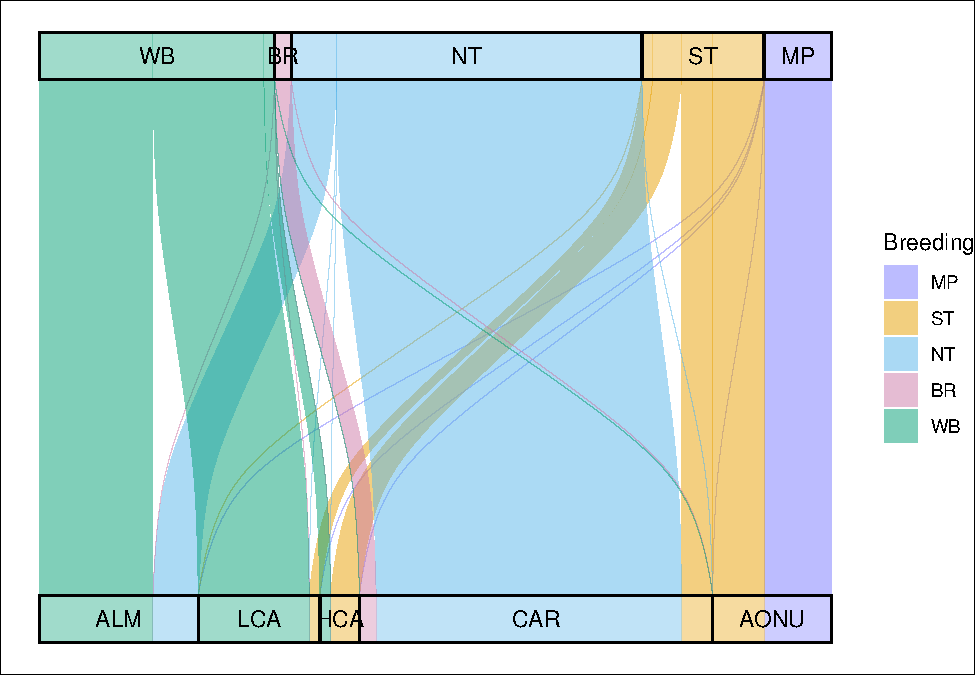
\includegraphics{Mignette_files/figure-latex/unnamed-chunk-23-1.pdf}

\hypertarget{supplemental}{%
\chapter{Supplement: Avian abundance data and genetic breeding nodes}\label{supplemental}}

This supplementary section provides more detailed information outside the scope of \texttt{mignette}. Specifically, the code here goes into details of using avian abundance data and genetic populations from a genoscape.

\hypertarget{breeding-nodes}{%
\section{Breeding nodes}\label{breeding-nodes}}

Delineating breeding nodes is necessary for our migratory network model for both 1) assignment among populations, and 2) specifying a region for relative abundance. Here, we show how breeding nodes can be delineated by genetically distinct populations on the breeding grounds. In this example, we'll show how to use \href{https://ebird.org/science/status-and-trends}{eBird Status and Trends} data to specify the breeding range and then use genetic data from admixture analyses to specify the spatial extent of the breeding nodes.

\hypertarget{ebirdst}{%
\subsection{ebirdst}\label{ebirdst}}

In our migratory network analyses, the \href{https://science.ebird.org/en/status-and-trends}{eBird Status and Trends} data is used to delineate the different stages of the annual cycle. Prior to doing anything with eBird Status and Trends data, you will need to download the \texttt{ebirdst} package, and then get access to the data. \textbf{You will need to follow the most up-to-date instructions from the \texttt{ebirdst} developers for getting the abundance data. Currently, that information is here: \url{https://ebird.github.io/ebirdst/}}

To download the package:

\begin{Shaded}
\begin{Highlighting}[]
\CommentTok{\# install.packages("remotes")}
\NormalTok{remotes}\SpecialCharTok{::}\FunctionTok{install\_github}\NormalTok{(}\StringTok{"CornellLabofOrnithology/ebirdst"}\NormalTok{)}
\end{Highlighting}
\end{Shaded}

Then, get access to \texttt{ebirdst} data at \url{https://ebird.org/st/request}. You will receive a key to download \texttt{ebirdst} data and you can enter that key in R:

\begin{Shaded}
\begin{Highlighting}[]
\NormalTok{ebirdst}\SpecialCharTok{::}\FunctionTok{set\_ebirdst\_access\_key}\NormalTok{(}\StringTok{"XXXXX"}\NormalTok{)}
\end{Highlighting}
\end{Shaded}

where \texttt{"XXXXX"} is the key.

By following instructions from the \texttt{ebirdst} developers, you can obtain polygons of the breeding and nonbreeding ranges of avian species (see \url{https://ebird.github.io/ebirdst/} for details).

\hypertarget{creating-the-genoscape}{%
\subsection{Creating the genoscape}\label{creating-the-genoscape}}

A genoscape is the collection of genetically distinct populations that make up a species' range \citep{ruegg2021american}. Typically, for migratory species, the genoscape describes this population structure on the breeding range because the nonbreeding populations can can contain individuals from different breeding populations.

We will outline the main genoscape creation steps here, but full instructions on creating a genoscape map can be found in Eric Anderson's Github project \href{https://github.com/eriqande/make-a-BGP-map}{Make a Bird Genoscape Project map}. The input data needed for a genoscape are:

\begin{itemize}
\tightlist
\item
  Individual Q-value matrix
\item
  Lat/lon matrix of individuals
\item
  Breeding range polygon
\end{itemize}

The Q-value matrix is obtained from individual admixture analyses (e.g.~Structure, Admixture, \texttt{snmf} fuction from the LEA R-package). Latitude/longitude coordinates are for the individual samples used in the Q-value matrix. Breeding range polygons can be obtained from \texttt{ebirdst} (see previous section).

The \texttt{amre\_breeding\_data} data set provides admixture results (Q-values) for five genetic clusters for American Redstart \citep{desaix2023low} and metadata for the sampled individuals.

\begin{Shaded}
\begin{Highlighting}[]
\FunctionTok{library}\NormalTok{(mignette)}
\NormalTok{Q\_matrix }\OtherTok{\textless{}{-}}\NormalTok{ mignette}\SpecialCharTok{::}\NormalTok{amre\_breeding\_data }\SpecialCharTok{\%\textgreater{}\%}
\NormalTok{  dplyr}\SpecialCharTok{::}\FunctionTok{select}\NormalTok{(WB, BR, NT, ST, MP) }\SpecialCharTok{\%\textgreater{}\%}
  \FunctionTok{as.matrix}\NormalTok{()}

\NormalTok{coords }\OtherTok{\textless{}{-}}\NormalTok{ mignette}\SpecialCharTok{::}\NormalTok{amre\_breeding\_data }\SpecialCharTok{\%\textgreater{}\%}
\NormalTok{  dplyr}\SpecialCharTok{::}\FunctionTok{select}\NormalTok{(Lon, Lat) }\SpecialCharTok{\%\textgreater{}\%}
  \FunctionTok{as.matrix}\NormalTok{()}
\end{Highlighting}
\end{Shaded}

The larger data objects in \texttt{mignette} are stored in \texttt{extdata}:

\begin{Shaded}
\begin{Highlighting}[]
\NormalTok{breeding\_range }\OtherTok{\textless{}{-}} \FunctionTok{system.file}\NormalTok{(}\StringTok{"extdata"}\NormalTok{, }\StringTok{"amre\_breeding\_range.Rds"}\NormalTok{, }\AttributeTok{package =} \StringTok{"mignette"}\NormalTok{)}
\NormalTok{breeding\_range }\OtherTok{\textless{}{-}}\NormalTok{ terra}\SpecialCharTok{::}\FunctionTok{vect}\NormalTok{(breeding\_range)}
  
\NormalTok{breeding\_range\_st }\OtherTok{\textless{}{-}}\NormalTok{ sf}\SpecialCharTok{::}\FunctionTok{st\_as\_sf}\NormalTok{(breeding\_range) }\CommentTok{\# tess3Q\_map\_rasters function requires sf objects, not terra}
\end{Highlighting}
\end{Shaded}

We will also specify custom colors to correspond to the published genoscape.

\begin{Shaded}
\begin{Highlighting}[]
\NormalTok{cluster\_colors }\OtherTok{\textless{}{-}}  \FunctionTok{c}\NormalTok{(}
  \StringTok{\textasciigrave{}}\AttributeTok{ST}\StringTok{\textasciigrave{}} \OtherTok{=} \StringTok{"\#e69f00"}\NormalTok{, }\CommentTok{\# orange/Southern Temperate}
  \StringTok{\textasciigrave{}}\AttributeTok{BR}\StringTok{\textasciigrave{}} \OtherTok{=} \StringTok{"\#cc79a7"}\NormalTok{, }\CommentTok{\# pink/Basin Rockies (BR)}
  \StringTok{\textasciigrave{}}\AttributeTok{NT}\StringTok{\textasciigrave{}} \OtherTok{=} \StringTok{"\#56b4e9"}\NormalTok{, }\CommentTok{\# light blue/Northern Temperate (NT)}
  \StringTok{\textasciigrave{}}\AttributeTok{WB}\StringTok{\textasciigrave{}} \OtherTok{=} \StringTok{"\#009e73"}\NormalTok{, }\CommentTok{\# green/Western Boreal (WB)}
  \StringTok{\textasciigrave{}}\AttributeTok{MP}\StringTok{\textasciigrave{}} \OtherTok{=} \StringTok{"\#7979ff"} \CommentTok{\# dark blue/Maritime Provinces (MP)}
\NormalTok{) }
\end{Highlighting}
\end{Shaded}

We will use a \href{https://github.com/eriqande/TESS3_encho_sen}{modified version of the \texttt{tess3r} package} to create the genoscape rasters.

\begin{Shaded}
\begin{Highlighting}[]
\CommentTok{\# remotes::install\_github("eriqande/TESS3\_encho\_sen")}
\NormalTok{amre\_genoscape }\OtherTok{\textless{}{-}}\NormalTok{ tess3r}\SpecialCharTok{::}\FunctionTok{tess3Q\_map\_rasters}\NormalTok{(}
  \AttributeTok{x =}\NormalTok{ Q\_matrix,}
  \AttributeTok{coord =}\NormalTok{ coords,}
  \AttributeTok{map.polygon =}\NormalTok{ breeding\_range\_st,}
  \AttributeTok{window =}\NormalTok{ sf}\SpecialCharTok{::}\FunctionTok{st\_bbox}\NormalTok{(breeding\_range\_st),}
  \AttributeTok{resolution =} \FunctionTok{c}\NormalTok{(}\DecValTok{300}\NormalTok{,}\DecValTok{300}\NormalTok{), }\CommentTok{\# if you want more cells in your raster, set higher}
  \AttributeTok{col.palette =}\NormalTok{ tess3r}\SpecialCharTok{::}\FunctionTok{CreatePalette}\NormalTok{(cluster\_colors, }\FunctionTok{length}\NormalTok{(cluster\_colors)), }
  \AttributeTok{method =} \StringTok{"map.max"}\NormalTok{, }
  \AttributeTok{interpol =}\NormalTok{ tess3r}\SpecialCharTok{::}\FunctionTok{FieldsKrigModel}\NormalTok{(}\DecValTok{10}\NormalTok{),  }
  \AttributeTok{main =} \StringTok{"Ancestry coefficients"}\NormalTok{,}
  \AttributeTok{xlab =} \StringTok{"Longitude"}\NormalTok{, }
  \AttributeTok{ylab =} \StringTok{"Latitude"}\NormalTok{, }
  \AttributeTok{cex =}\NormalTok{ .}\DecValTok{4}
\NormalTok{)}
\FunctionTok{names}\NormalTok{(amre\_genoscape) }\OtherTok{\textless{}{-}} \FunctionTok{colnames}\NormalTok{(Q\_matrix)}
\NormalTok{amre\_genoscape }\OtherTok{\textless{}{-}}\NormalTok{ terra}\SpecialCharTok{::}\FunctionTok{rast}\NormalTok{(amre\_genoscape) }\CommentTok{\# convert from rasterbrick to spatRaster}
\FunctionTok{crs}\NormalTok{(amre\_genoscape) }\OtherTok{\textless{}{-}} \StringTok{"EPSG:4326"} \CommentTok{\# Set CRS projection}
\end{Highlighting}
\end{Shaded}

Check out the resulting genoscape:

\begin{Shaded}
\begin{Highlighting}[]
\FunctionTok{plot}\NormalTok{(amre\_genoscape)}
\end{Highlighting}
\end{Shaded}

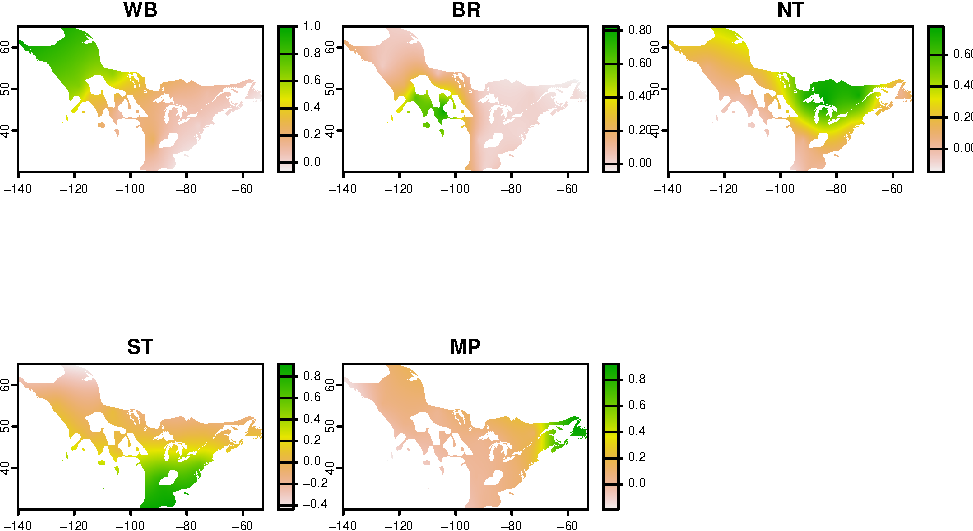
\includegraphics{Mignette_files/figure-latex/unnamed-chunk-25-1.pdf}

\textbf{STOP}

The rasters for the genoscape are all that are needed for obtaining information on relative abundance for the different populations. You can continue on to the \protect\hyperlink{abundance}{relative abundance chapter} if you are ready to do that with the genoscape. Or if you still need to create the wintering nodes, check out the next chapter on \protect\hyperlink{wintering}{wintering nodes}. The following section is not necessary for the migratory network but details how to covert genoscape rasters to polygons if the \texttt{mignette} user is interested in doing so.

\hypertarget{genoscape-polygons}{%
\subsection{Genoscape polygons}\label{genoscape-polygons}}

Using the genoscape rasters we will convert them to polygons, using the handy \texttt{scape\_to\_shape()} function. The \texttt{prob\_threshold} parameter specifies the value to determine if a raster cell is included in the polygon for that genoscape. This value should be customized for different species to check for overlap of genoscape polygons, which is not desirable. Setting too high of a threshold will create very small breeding nodes, while too low of a threshold will result in large, overlapping breeding nodes.

Check out the polygons

\begin{Shaded}
\begin{Highlighting}[]
\NormalTok{genoscape\_polygons }\OtherTok{\textless{}{-}}\NormalTok{ mignette}\SpecialCharTok{::}\FunctionTok{scape\_to\_shape}\NormalTok{(}\AttributeTok{x =}\NormalTok{ amre\_genoscape, }
                                               \AttributeTok{prob\_threshold =} \FloatTok{0.5}\NormalTok{)}
\end{Highlighting}
\end{Shaded}

\begin{verbatim}
## Spherical geometry (s2) switched off
\end{verbatim}

\begin{Shaded}
\begin{Highlighting}[]
\FunctionTok{ggplot}\NormalTok{() }\SpecialCharTok{+}
  \FunctionTok{geom\_sf}\NormalTok{(}\AttributeTok{data =}\NormalTok{ genoscape\_polygons,}\AttributeTok{alpha =} \FloatTok{0.75}\NormalTok{, }\FunctionTok{aes}\NormalTok{(}\AttributeTok{fill =}\NormalTok{ Cluster)) }\SpecialCharTok{+}
  \FunctionTok{scale\_fill\_manual}\NormalTok{(}\AttributeTok{values =}\NormalTok{ cluster\_colors) }\SpecialCharTok{+}
  \FunctionTok{theme\_bw}\NormalTok{()}
\end{Highlighting}
\end{Shaded}

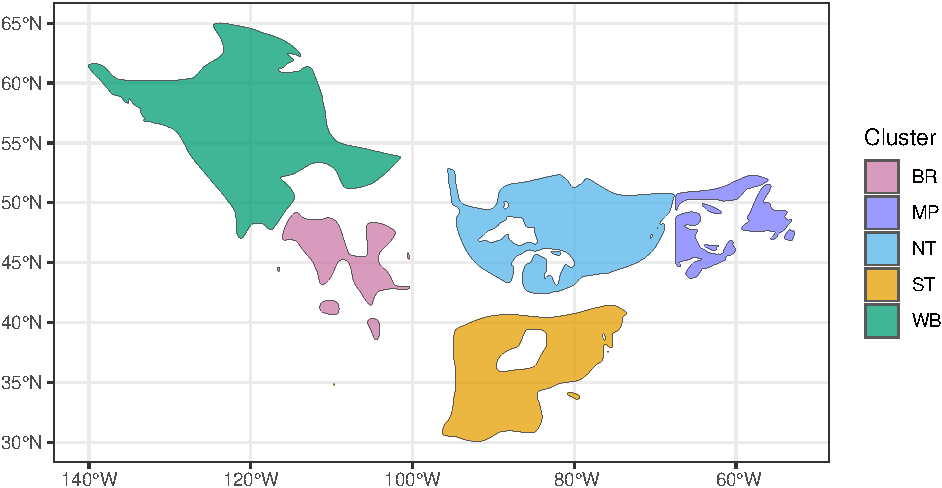
\includegraphics[width=0.7\linewidth]{Mignette_files/figure-latex/unnamed-chunk-27-1}

  \bibliography{book.bib,packages.bib}

\end{document}
